\documentclass{thisbook}

\usepackage{svg} % automatically convert svg and include
\usepackage{pgfplots} \pgfplotsset{compat=1.10} % also includes tikz


%%%%%%%%%% BOOK INFORMATION %%%%%%%%%%
\newcommand{\authorname}{Everyone who contributed.}
\newcommand{\booktitle}{Mathematical Analysis~2}
% \newcommand{\subtitle}{Lecture notes 2021/22}
\newcommand{\sourcelink}{\href{https://github.com/oliver-butterley/ma2}{\texttt{github.com/oliver-butterley/ma2}}}
\newcommand{\editionyear}{2021}

\title{\booktitle}
\author{\authorname}
    
\theoremstyle{plain}
\newtheorem{theorem}{Theorem}[chapter]
\newtheorem*{theorem*}{Theorem}
\newtheorem{task}[theorem]{Task} % Environment for exercises
\newtheorem{lemma}[theorem]{Lemma}
\newtheorem*{lemma*}{Lemma}
\theoremstyle{definition}
\newtheorem{example}[theorem]{Example}
\newtheorem*{example*}{Example}
\newtheorem{definition}[theorem]{Definition}
\newtheorem*{definition*}{Definition}
\theoremstyle{remark}
\newtheorem{remark}[theorem]{Remark}
\newtheorem*{remark*}{Remark}
\newenvironment{solution}{\begin{proof}[Solution]}{\end{proof}} % Environment for solutions of tasks

% Highlighted versions of definition and theorem
\tcolorboxenvironment{definition}{
    colback=blue!5!white, 
    arc=2mm,  enhanced, frame hidden, oversize,
    left=2mm,right=2mm,top=1mm,bottom=1mm}
\tcolorboxenvironment{theorem}{
    colback=blue!5!white, 
    arc=2mm,  enhanced, frame hidden, oversize,
    left=2mm,right=2mm,top=1mm,bottom=1mm}

\colorlet{paleBlue}{blue!10!white}

\usepackage{style/options}

%%%%%%%%% mathematics helpers
\newcommand{\abs}[1]{\left|#1\right|}
\newcommand{\bC}{\mathbb{C}} % Complex numbers
\newcommand{\bN}{\mathbb{N}} % Natural numbers
\newcommand{\bR}{\mathbb{R}} % Real numbers
\newcommand{\norm}[1]{\left\|#1\right\|} % Norm
\renewcommand{\aa}{\mathbf{a}}
\newcommand{\bb}{\mathbf{b}}
\newcommand{\cc}{\mathbf{c}}
\newcommand{\ee}{\mathbf{e}}
\newcommand{\ff}{\mathbf{f}}
\renewcommand{\gg}{\mathbf{g}}
\newcommand{\hh}{\mathbf{h}}
\newcommand{\rr}{\mathbf{r}}
\newcommand{\uu}{\mathbf{u}}
\newcommand{\vv}{\mathbf{v}}
\newcommand{\ww}{\mathbf{w}}
\newcommand{\xx}{\mathbf{x}}
\newcommand{\yy}{\mathbf{y}}
\newcommand{\zz}{\mathbf{z}}
\newcommand{\aalpha}{\boldsymbol{\alpha}}
\newcommand{\littleo}[1]{o(#1)}
%%%%%%%%%


\begin{document}

\frontmatter
\pagestyle{empty}

% Half title page
% {
% 	\centering

% 	~

% 	\vspace{24pt}
% 	{\scshape\Huge \booktitle \par}
% }

% Title page
\begin{titlepage}
	\centering

	~

	\vspace{24pt}
	{\scshape\Huge \booktitle\par}
	\vspace{6pt}
	{\scshape\large \subtitle\par}
	\vspace{\stretch{1.25}}
	{\itshape\large by\par}
	\vspace{6pt}
	{\itshape\Large \authorname\par}
	\vspace{\stretch{6}}
	{\large \publisher\par}
\end{titlepage}

% Copyright page

{\small
\setlength{\parindent}{0em}\setlength{\parskip}{1em}

~

\vfill


\doclicenseIcon
This text is licensed under 
\doclicenseLongNameRef \ 
(\doclicenseNameRef).

You are free to 
\textbf{share} this work (copy and redistribute the material in any medium or format) 
and 
\textbf{adapt} this work (remix, transform, and build upon the material for any purpose, even commercially),
under the obligation of 
\textbf{attribution} (you must give appropriate credit)
and
\textbf{share alike} (if you remix, transform, or build upon the material, you must distribute your contributions under the same license as the original). 

This text may contain errors, inaccuracies and misleading ideas, the reader takes full responsibility for the consequences. 
Any resemblance to actual persons, living or dead, events or localities is entirely coincidental.

Typeset: \today

Source available at: \publisher{}
}

\chapter{Preface}
\lettrine{T}{his} text accompanies the course ``Mathematical Analysis 2'' taught at the University of Rome Tor Vergata in the department of engineering 2022--2025.
During these years the course was led by Oliver Butterley. 

The aim of this document is to concisely describe the fundamental details related to the material of the course.
They are aptly named as ``notes'' and are most likely not the comprehensive source of all relevant information.
We have easy access to a huge volume of resources and so here we will make connections to whatever is useful, whenever we can. 

These notes are merely written text whereas the central part of the course remains the time spent working with the material, be it doing exercises, discussing, doing calculations, etc. This is not text for memorising, this is text that aims to help us practice and become stronger thinkers.

This text is freely\footnote{Free both in the sense of \href{https://en.wikipedia.org/wiki/Gratis_versus_libre}{``free speech'' and ``free beer''}.} available at \href{https://github.com/oliver-butterley/ma2}{\textbf{github.com/oliver-butterley/ma2}}.
Everyone is encouraged to contribute improvements to the document during the progress of the course. 

Some of the text comes from previous years and from many other sources, some of the text came to be during the course.
The current version is the product of many people, in particular everyone who has made suggestions in class and pointed out errors or imprecisions and to everyone who suggested useful additional content.


% \cleardoublepage   
% % Make sure contents page starts on right-side page
\tableofcontents\thispagestyle{empty}\cleardoublepage%

\pagestyle{plain}

% !TeX root = ../main.tex
\chapter{Introduction}

\lettrine{W}{e} start by looking at examples which demonstrate some of the motives behind studying analysis in general.
%
\begin{example*}[Series]
  The geometric series
  \(S = 1 + \frac{1}{2} + \frac{1}{4} + \frac{1}{8} + \frac{1}{16} + \cdots\)
  can be summed by the following simple trick.
  Multiplying by \(2\) we obtain that
  \[
    2S = 2 + 1 + \frac{1}{2} + \frac{1}{4} + \frac{1}{8} + \frac{1}{16} + \cdots = 2+S
  \]
  and so \(S=2\).
  If we try to do the same to the sum
  \(T = 1 + 2 + 4 + 8 + 16 + \cdots\)
  we get the nonsensical answer
  \[
    2T = 2 + 4 + 8 + 16 + \cdots = T -1
  \]
  and so \(T = -1\).
  %
  Why should we trust the argument in the first case and not in the second?
\end{example*}


\begin{example*}[Interchanging sums]
  If we consider any matrix of numbers, for example,
  \[
    \begin{pmatrix}
      1 & 2 & 3 \\
      4 & 5 & 6 \\
      7 & 8 & 9
    \end{pmatrix}
  \]
  we can sum first the rows \(6 + 15 + 24 = 45\) or first the columns \(12 + 15 + 18 = 45\) to obtain the total sum of all numbers.
  This is the rule
  \[
    \sum_{j=1}^{m} \sum_{k=1}^{n} a_{jk} = \sum_{k=1}^{n} \sum_{j=1}^{m}  a_{jk}.
  \]
  We would like to believe that also \(\sum_{j=1}^{\infty} \sum_{k=1}^{\infty} a_{jk} = \sum_{k=1}^{\infty} \sum_{j=1}^{\infty}  a_{jk}\).
  However this doesn't work for the following matrix:
  \[
    \begin{pmatrix}
      1      & 0      & 0      & \cdots \\
      -1     & 1      & 0      & \cdots \\
      0      & -1     & 1      & \cdots \\
      \vdots & \vdots & \vdots & \ddots
    \end{pmatrix}.
  \]
  %
  We often want to swap the order of summing (or integrating) and often need to consider infinite sums (or integrals).
  When can we do this and can't we?
\end{example*}

\begin{example*}[Interchanging integrals]
  Let's try to integrate \(e^{-xy} - xye^{-xy}\) with respect to both \(x\) and \(y\).
  We would like to believe that
  \[
    \int_{0}^{\infty} \left[ \int_{0}^{1} (e^{-xy} - xye^{-xy}) \ dy \right] \ dx
    \overset{\text{\large\color{blue}?}}{=} \int_{0}^{1} \left[ \int_{0}^{\infty}  (e^{-xy} - xye^{-xy}) \ dx \right] \ dy.
  \]
  Since
  \( \int_{0}^{1} (e^{-xy} - xye^{-xy}) \ dy = {\left[ye^{-xy}\right]}_{y=0}^{1} = e^{-x}\),
  the left-hand side is
  \( \int_{0}^{\infty} e^{-x} \ dx = {\left[ -e^{-x} \right]}_{0}^{\infty} = 1 \).
  However, since
  \( \int_{0}^{\infty}  (e^{-xy} - xye^{-xy}) \ dx = {\left[ xe^{-xy} \right]}_{x=0}^{\infty} = 0\),
  the right-hand side is \(\int_{0}^{1} 0 \ dx = 0\).
  So how do we know when to trust the interchange of intervals?
\end{example*}


\begin{example*}[interchanging limits]
  We could easily believe that
  \[
    \lim_{x\to 0}\lim_{y\to 0} \frac{x^2}{x^2 + y^2}
    \overset{\text{\large\color{blue}?}}{=}
    \lim_{y\to 0}\lim_{x\to 0} \frac{x^2}{x^2 + y^2}.
  \]
  However \(\lim_{y\to 0} \frac{x^2}{x^2 + y^2} = \frac{x^2}{x^2 + 0} = 1 \) and so the left-hand side is \(1\)
  whereas \(\lim_{x\to 0} \frac{x^2}{x^2 + y^2} = \frac{0}{0 + y^2} = 0\) so the right-hand side is \(0\).
  What does the graph of this function look like?
  This example shows that the interchange of limits is untrustworthy. Under what circumstances is it legitimate?
\end{example*}

We need to be rigorous in our logic otherwise, as we have seen in these examples, the conclusions can be erroneous and the difficulties are often subtle.

\subsection*{Curves of constant width}
%
\begin{figure}[htb]
  \centering
  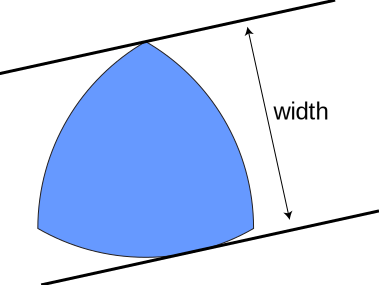
\includegraphics{reuleaux.pdf}
  \caption{The Reuleaux triangle is a curve of constant width.}%
  \label{fig:reuleaux}
\end{figure}
%
The above examples are calculus based but it is worthwhile to consider a real world application of the rigour and reasoning we aspire to.
Suppose we are organising the production facilities which manufacture a component that is round (maybe a rocket body, maybe a propellant tube, etc.).
\begin{samepage}
  As part of the production it is important to have a procedure which guarantees that the fabrication is done to the correct tolerance.
  The idea proposed is:
  \begin{quotation}
    ``We measure the width from all angles to confirm that the manufactured component is correct.''
  \end{quotation}
\end{samepage}
This is a two-dimensional problem in the sense we assume that the object is a closed curve in \(\bR^2\).
For a given angle we define the width of this curve to be the smallest distance between two parallel lines which touch the curve in a single point but never cross it (one each side of the curve).
We say that the curve has constant width if this width is equal from every direction.
This is just what we would check using calipers on a part and rotating.
The following statement is intuitive and true.
\begin{theorem*}
  A circle has constant width.
\end{theorem*}
\noindent
However the converse is not true, indeed the following is true.
\begin{theorem*}
  There exist constant width curves which are not circles.
\end{theorem*}
\noindent
This can be proved by constructing many such curves, for example the \href{https://en.wikipedia.org/wiki/Reuleaux_triangle}{Reuleaux triangle}. Indeed there are such curves which look similar to regular polygons but still have constant width.


% \footnotetext{
%   Source of Figure~\ref{fig:reuleaux}: 
%   \url{https://commons.wikimedia.org/wiki/File:Reuleaux_supporting_lines.svg}
%   }



\subsection*{MA2 versus MA1}

Much of what we do in this course builds on ideas established in Mathematical Analysis 1.
In particular many of the ideas are extended to the higher dimensional setting. See Table~\ref{tab:2versus1}.

\begin{table}
  \centering
  \begin{tabular}{r | l} % chktex 44
    \textbf{Mathematical Analysis 1}
     &
    \textbf{Mathematical Analysis 2}  \\
    \midrule
    Sequences \& series of numbers
     &
    Sequences \& series  of functions \\
    \(a_1, a_2, a_3,\ldots \)
     &
    \(f_1(x), f_2(x), f_3(x),\ldots \)
    \\
    \(\sum_{n=0}^{\infty} a_n\)
     &
    \(\sum_{n=0}^{\infty} f_n(x)\)
    \\
    \midrule
    (Functions) \(f:\bR \to \bR\)
     &
    \(f:\bR^n \to \bR\) (Scalar fields)
    \\
     &
    \(\mathbf{f}:\bR^n \to \bR^n\) (Vector fields)
    \\
     &
    \(\boldsymbol{\alpha}:\bR \to \bR^n\) (Paths)
    \\
    \midrule
    (Derivative) \( f'(x) = \frac{df}{dx}(x)\)
     &
    \( \frac{\partial f}{\partial x_j}(x_1,\ldots,x_n)\) (Partial derivatives)
    \\
     &
    \(\nabla f\) (Gradient)
    \\
     &
    \(D_v f\) (Directional derivative)
    \\
     &
    \(\boldsymbol{\alpha}'\) (Derivative of path)
    \\
     &
    \(Df\) (Jacobian matrix)
    \\
     &
    \(\nabla \cdot \ff\) (Divergence)
    \\
     &
    \(\nabla \times \ff\) (Curl)
    \\
    \midrule
    (Extrema) \(\sup_{x\in \bR} f(x)\)
     &
    \(\sup_{x\in \bR^n} f(x)\) (Extrema)
    \\
     &
    Lagrange multiplier method
    \\
    \midrule
    Integral \(\int_{a}^{b} f(x) \ dx\)
     &
    Multiple integral
    \\
     &
    Line integral
    \\
     &
    Surface integral
  \end{tabular}
  \caption{Ma2 versus MA1}%
  \label{tab:2versus1}
\end{table}


\subsection*{Suggested further reading}

\begin{itemize}
  \item ``Analysis 1'' by Terence Tao.
        (Particularly \S 1.2 ``Why Analysis?'' and Appendix A ``The basics of mathematical logic'').
\end{itemize}

\mainmatter
% !TeX root = ../main.tex
\chapter{Sequences \& series of functions}

\lettrine{A}{nalogously} to sequences of numbers we can consider a sequence of functions \(f_0(x)\), \(f_1(x)\), \(f_2(x)\), \(f_3(x)\), etc.
Often it is convenient to write such a sequence as \({\{ f_n(x)\}}_{n\in \mathbb{N}}\).
For example, the following are sequences of functions.
\begin{itemize}
  \item \(f_1(x) = x^2, f_2(x)=x^4, f_3(x)=x^6,\ldots \)
  \item \(f_1(x) = e^x, f_2(x)=e^{2x}, f_3(x)=e^{3x},\ldots \)
  \item \(f_n(x) = n \exp \left( - \frac{1}{2}n^2 x^2 \right)\)
\end{itemize}

Note that in the first case we could have instead written \(f_n(x) = x^{2n}\) and in the second case we could have written  \(f_n(x) = e^{nx}\).
The natural number \(n\) is called the index.
Typically the index of the sequence starts from \(n=0\) or \(n=1\) but that's not essential.
The index doesn't need to be \(n\), any other letter, or indeed symbol, can be used.


\section{Convergence \& continuity}

We start by recalling the notion of convergence for sequences of numbers.

\begin{definition}
  A sequence of numbers  \(a_1, a_2, a_3,\ldots \) is said to \emph{converge} to \(a\) if, for each \(\epsilon>0\), exists \(N\in \mathbb{N}\) such that \(|a_n - a| < \epsilon\) whenever \(n\geq N\).
\end{definition}
%
\noindent
If a sequence \({\{a_n\}}_{n}\) converges to \(a\) then we write \(a_n \to a\) (as \(n\to \infty\)).
For sequences of functions we will need to consider two different notions of convergence.
In order to understand this difficulty let us consider the following example.

\begin{example*}
  Consider the sequence \(f_n(x) = x^n\) for \(x\in (0,1)\).
  For each \(x\in (0,1)\) we see that \(f_n(x) \to 0\).
  On the other hand, for each \(n\), \(2^{\frac{1}{n}}\in (0,1)\) and \(f_n(2^{\frac{1}{n}}) = \frac{1}{2}\).
\end{example*}


\begin{figure}
  \begin{center}
    \includegraphics{sequence-xn.pdf}
    \caption{The sequence of functions \(f_n(x)= x^n\).}
  \end{center}
\end{figure}

\noindent
Up until now we haven't mentioned the domain of the functions in the sequence but to proceed we need to be make this detail rigorous.
We will write that ``\({\{f_n(x)\}}_{n}\) is a sequence of functions on \(D\subset \bR\)'' to mean that there is a fixed \(D\subset \bR\) and, for each \(n\in \bN\), \(f_{n}\) is a function with domain \(D\) (i.e., \(f_n : D \to \bR\)).


\begin{definition}[pointwise convergence]
  Let \(D\subset \mathbb{R}\),
  let \(f_n(x)\) be a sequence of functions on \(D\)
  and let \(f(x)\) be a function on \(D\).
  If \(f_n(x) \to f(x)\) for each \(x\in D\) we say that \(f_n\) is \emph{pointwise convergent} to \(f\).
\end{definition}

\begin{definition}[uniform convergence]
  Let \(f_n(x)\) be a sequence of functions on \(D\subset \mathbb{R}\)
  and let \(f(x)\) be a function on \(D\).
  If, for each \(\epsilon>0\), there exists \(N\) such that for every \(n\geq N\) and every \(x\in D\), \(|f_n(x) - f(x)| < \epsilon\) then we say that \(f_n\) is \emph{uniformly convergent} to \(f\).
\end{definition}

\begin{example*}
  Show that \(f_n(x) = x^n\) converges uniformly on \((0,\frac{1}{2})\).
\end{example*}

\begin{solution}
  We observe that it converges pointwise to the constant function \(f(x)=0\).
  We also observe that \(|f_n(x) - f(x) | \leq \frac{1}{2^n}\) for all \(x\in (0,\frac{1}{2})\).
  This means that, for every \(\epsilon>0\), if we can choose \(N=-\log_{2}\epsilon\) then \(|f_n(x) - f(x) | \leq \epsilon\) whenever \(n\geq N\).
\end{solution}

\begin{definition}
  Let \(f(x)\) be a functions on \(D\subset \mathbb{R}\).
  We say that \(f\) is \emph{continuous} at \(p\in D\) if, for each \(\epsilon>0\), there is \(\delta >0\) such that \(|f(x)-f(p)| <\epsilon\) whenever \(x\in D\), \(|x-p| <\delta\).
  We say that \(f\) is \emph{continuous on \( D\)} if \(f\) is continuous at every \(p\in D\).
\end{definition}

\begin{figure}
  \begin{center}
    \includegraphics{sequence-arctan.pdf}
    \caption{The sequence of functions \(f_n(x)= \arctan(nx)\).}
  \end{center}
\end{figure}

It is natural to consider a sequence of continuous functions which converge and ask if the function they converge to is continuous.
What about the sequence of functions \(f_n(x) = \arctan (nx)\)?

\begin{theorem}%
  \label{thm:continuous-limit}
  Suppose that \(f_n \to f\) uniformly on \(D\) and that the \(f_n\) are continuous on \(D\).
  Then \(f\) is continuous on \(D\).
\end{theorem}


\begin{proof}
  Let \(p\in D\).
  Uniform convergence means that, for each \(\epsilon>0\), there exists \(N\) such that for every \(n\geq N\) and every \(x\in D\), \(|f_n(x) - f(x)| < \frac{\epsilon}{3}\).
  By continuity of \(f_N(x)\) at \(x=p\), there is a \(\delta >0\) such that \(|f_N(x)-f_N(p)| < \frac{\epsilon}{3} \) whenever \(x\in D\), \(|x-p| <\delta\).
  Since
  \[
    | f(x) - f(p) | = |f(x) - f_N(x) + f_N(x) - f_N(p) + f_N(p) - f(p) | \]
  this means that, for all \(|x-p| <\delta\),
  \[
    \begin{aligned}
      | f(x) - f(p) | & \leq   |f(x) - f_N(x)| + |f_N(x) - f_N(p)| + |f_N(p) - f(p) | \\
                      & < 3 \frac{\epsilon}{3} = \epsilon.
    \end{aligned}
  \]
  This proves the continuity of \(f\) at \(p\). Since \(p\in D\) is arbitrary this shows the continuity of \(f\) on \(D\).
\end{proof}


Recall that integrals are defined rigorously using the notion of a step functions.

\begin{theorem}%
  \label{thm:limit-of-integral}
  Suppose that \(f_n\) are continuous functions on \([a,b] \subset \mathbb{R}\), uniformly convergent to \(f\).
  Then
  \[
    \lim_{n\to \infty} \int_{a}^{b} f_n(x) \ dx = \int_{a}^{b} f(x) \ dx.
  \]
\end{theorem}

\begin{proof}
  The uniform convergence implies that for each \(\epsilon>0\), there exists \(N\) such that for every \(n\geq N\) and every \(x\in D\), \(|f_n(x) - f(x)| <  \frac{\epsilon}{b-a}\).
  This means that
  \[
    \begin{aligned}
      \Big| \int_{a}^{b} f_n(x) \ dx - \int_{a}^{b} f(x) \ dx \Big|
       & \leq \int_{a}^{b} | f_n(x) - f(x) | \ dx    \\
       & \leq (b-a) \frac{\epsilon}{b-a} = \epsilon.
    \end{aligned}
  \]
  This shows that \(\int_{a}^{b} f_n(x) \ dx \to  \int_{a}^{b} f(x) \ dx\).
\end{proof}


\subsection*{Series of functions}



Recall that for a sequence \({\{a_n\}}_{n}\) of numbers,
the series \(\sum_{n}a_n\) is the sequence \({\{\sum_{k=1}^{n}a_k\}}_{n}\) of numbers (the partial sums).
We say that the series  \(\sum_{n}a_n\) is convergent if \({\{\sum_{k=1}^{n}a_k\}}_{n}\) is convergent.



\begin{definition}
  Let \(\{f_n\}\) be a sequence of functions.
  We say that the series \(\sum_{n} f_n\)
  \begin{itemize}
    \item   is \emph{pointwise convergent} if
          \(\sum_{k=1}^{n} f_k(x)\) is pointwise convergent,
    \item   is \emph{uniformly convergent} if
          \(\sum_{k=1}^{n} f_k(x)\) is uniformly convergent.
  \end{itemize}
\end{definition}


\begin{theorem}
  Suppose that the series \(\sum_{n} f_n\) is uniformly convergent to \(g\) on \(D\) and the \(f_n\) are continuous on \(D\).
  Then \(g\) is continuous on \(D\).
\end{theorem}

\begin{proof}
  If the \(f_k\) are continuous then the \(\sum_{k=1}^{n} f_k\) are continuous.
  This means that Theorem~\ref{thm:continuous-limit} applies.
\end{proof}

\begin{theorem}
  Suppose that the series \(\sum_{n} f_n\) is uniformly convergent to \(g\) and the \(f_n\) are continuous.
  Then
  \[
    \lim_{n\to\infty} \int_{a}^{b}  \sum_{k=1}^{n} f_k(x)  \ dx = \int_{a}^{b} g(x) \ dx.
  \]
\end{theorem}

\begin{proof}
  Again, that the \(f_k\) are continuous means that the \(\sum_{k=1}^{n} f_k\) are continuous.
  This means that Theorem~\ref{thm:limit-of-integral} applies.
\end{proof}

Here and subsequently it is convenient to recall several commons tests which are useful for proving convergence:
\href{https://en.wikipedia.org/wiki/Ratio_test}{ratio test},
\href{https://en.wikipedia.org/wiki/Root_test}{root test},
\href{https://en.wikipedia.org/wiki/Direct_comparison_test}{comparison test},
\href{https://en.wikipedia.org/wiki/Alternating_series_test}{alternating series test},
\href{https://en.wikipedia.org/wiki/Integral_test_for_convergence}{integral test for convergence}.
%
For series of functions we have the following test for convergence.

\begin{theorem}[Weierstrass M-test]
  Suppose that \({\{f_n\}}_n\) is a sequence of functions on \(D\), that \({\{M_n\}}_n\) is a sequence of positive numbers
  and that \(|f_n(x)|\leq M_n\).
  If \(\sum_{n=0}^{\infty}M_n\) is convergent then the series \(\sum_{n=0}^{\infty}f_n\) converges absolutely and uniformly on \(D\).
\end{theorem}

\begin{proof}
  By the comparison test \(\sum |f_n(x)| \) is convergent for all \(x\in D\).
  I.e., for each \(x\) the series \(\sum f_n(x) \) is absolutely convergent and so we let \(f(x)\) be the limit.
  We compute
  \[
    \Big|f(x) - \sum_{k=1}^{n} f_k(x)  \Big|
    =
    \Big|\sum_{k=n+1}^{\infty} f_k(x)  \Big|
    \leq \sum_{k=n+1}^{\infty} |f_k(x)|
    \leq  \sum_{k=n+1}^{\infty} M_k.
  \]
  As \(\sum_{n}M_n\) is convergent this last expression tends to \(0\) as \(k\to \infty\).
  This estimate is independent of \(x\).
\end{proof}

\section{Power series}

\begin{definition}
  Let \({\{a_n\}}_{n}\) be a series of numbers and let \(c\) be a number.
  The series
  \(\sum_{n} a_n {(x-c)}^n\)
  is called a \emph{power series} (centred at \(c\)).
\end{definition}
Typically the power series will converge for some \(x\) and diverge for other \(x\).
We could permit \(x\) to be a complex number and the entire work of this section holds verbatim.
However, for the present purposes we will assume that \(x \in \bR\) and that the coefficients \(a_n \in \bR\) and that \(c\in \bR\).
To simplify formulae we will often work with the case that \(c=0\) since we can always transform a given problem to this special case.

\begin{example*}
  Let \(a_n = 2^{-n}\).
  The power series \(\sum_{n} a_n x^n = \sum_{n}\frac{x^n}{2^n}\) is convergent when \(\abs{x}<2\) and divergent  when \(\abs{x} > 2\).
  To see this we apply the root test and observe that  \(\lim_{n\to\infty}{\big(2^{-n}\abs{x}^n \big)}^{\frac{1}{n}}=\frac{\abs{x}}{2}\).
\end{example*}

\begin{example*}
  Let \(a_n = \frac{1}{n!}\).
  The power series \(\sum_{n}\frac{x^n}{n!}\) is convergent for all \(x\).
  To see this we use the ratio test and observe that  \(\abs{\frac{x^{n+1}}{(n+1)!} }/ \abs{\frac{zx^n}{n!}} = \frac{\abs{x}}{n+1}\) and that \(\lim_{n\to\infty} \frac{\abs{x}}{n+1} = 0 \) for any \(x\).
\end{example*}


\section{Radius of convergence}

A key notion is determining exactly the domain on which a power series converges.

\begin{theorem}[uniformly convergent power series]
  Suppose that \(\sum_{n}a_n x^n\) converges for some \(x=x_0 \neq 0\).
  Let \(R<\abs{x_0}\).
  Then the series is uniformly and absolutely convergent for all \(x\) such that \(\abs{x}\leq R\).
\end{theorem}

\begin{proof}
  Since \(\sum_n a_n x_0^n\) is convergent there exists  \(M>0\) such that, for all \(n\), \(\abs{a_n x_0^n} \leq M\).
  Observe that
  \[
    \abs{a_n x^n} = \abs{a_n x_0^n} \ \abs{\tfrac{x}{x_0}}^n \leq M \tfrac{R^n}{\abs{x_0}^n}.
  \]
  The series
  \(\sum_n M \frac{R^n}{\abs{x_0}^n}\) is a geometric sum and so convergent.
  Consequently, by the M-test, the series is uniformly and absolutely convergent when \(\abs{x}\leq R\).
\end{proof}

\begin{theorem}[radius of convergence]%
  \label{thm:radius-of-convergence}
  Suppose exists  \(x_1,x_2 \neq 0\) such that \(\sum_n a_n x_1^n\) is convergent and \(\sum_n a_n x_2^n\) is divergent.
  Then exists \(r>0\) such that \(\sum_n a_n x^n\) is convergent for \(\abs{x}<r\) and divergent for \(\abs{x}>r\).
\end{theorem}

\begin{proof}
  Let \(A\) be the set of real numbers for which \(\sum_n a_n x^n\) is convergent and
  let \(r\) be the least upper bound of \(A\).
  The series  \(\sum_n a_n x^n\) is convergent whenever \(\abs{x}<r\).
  If \(\abs{x}>r\) and \(\sum_n a_n x^n\) is convergent then this contradicts the definition of \(A\) and so  \(\sum_n a_n x^n\) is divergent for \(\abs{x}>r\).
\end{proof}

In the above paragraphs we worked with the case \(c=0\) but all of these notions hold for the general \(c\in \bR\). Consequently Theorem~\ref{thm:radius-of-convergence} implies that the series is convergent on an interval \((c-r,c+r) = \{x:\abs{x-c}<r\}\) but divergent when \(\abs{x-c}>r\).
The convergence for the sequence for \(x=c-r\) and \(x=c+r\) must be manually checked and can differ for the left and right end points.

\begin{definition}
  This \(r\) is the \emph{radius of convergence} of the series \(\sum_n a_n {(x-c)}^n\).
\end{definition}

We use the following convention:
if \(\sum_n a_n x^n\) converges for all \(x\in \bC\) we say the radius of convergence is \(\infty\);
if \(\sum_n a_n x^n\) doesn't converge except  \(x=0\) we say the radius of convergence is \(0\).
All of the above concerning power series holds verbatim for \(x\) a complex number and so ``radius'' is more meaningful since it truly corresponds to a disk in the complex plane.




\section{Integrating \& differentiating power series}

Let \(a_n \in \bR\), \(x\in \bR\).
If the series \(\sum_n a_n x^n\) converges we define the function \(f(x) = \sum_{n=0}^{\infty} a_n x^n\).
In general exchanging limits with derivatives and integrals is problematic but for power series the situation is good.

\begin{theorem}[integrating power series]%
  \label{thm:integrate-power}
  Suppose that, for \(x\in (-r,r)\), the series  \(f(x) = \sum_{n=0}^{\infty} a_n x^n\) is convergent.
  Then \(f(x)\) is continuous and \(\int_0^x f(y) \ dy = \sum_{n=0}^{\infty} \frac{a_n}{n+1} x^{n+1}\).
\end{theorem}

\begin{proof}
  Let \(\abs{x}<R<r\).
  Observe that the series is uniformly convergent for \(y\in[-R,R]\).
  This means that \(f(x)\) is continuous and so we can interchange limit and integral,
  \[
    \int_0^x f(y) \ dy
    = \sum_{n=0}^{\infty} \int_0^x  {a_n} x^{n}
    = \sum_{n=0}^{\infty} \frac{a_n}{n+1} x^{n+1}.
  \]
\end{proof}

\begin{theorem}[differentiating power series]%
  \label{thm:differentiate-power}
  Suppose that, for \(x\in (-r,r)\), the series  \(f(x) = \sum_{n=0}^{\infty} a_n x^n\) is convergent.
  Then \(f(x)\) is differentiable and \(f'(x) =\sum_{n=1}^{\infty} n a_n x^{n-1}\), convergent for \(x\in (-r,r)\).
\end{theorem}

\begin{proof}
     Let \(\abs{x}<R<r\). 
     Observe that
          \[
            \sum_{n=1}^{\infty} n a_n x^{n-1}    = \sum_{n=1}^{\infty} a_n R^{n} \cdot \frac{n}{R} \cdot \frac{{x}^{n-1}}{R^{n-1}}.
            \]
     Since \(\sum_{n=1}^{\infty} a_n R^n\) is absolutely convergent and \(  \frac{n}{R}  \cdot {( \frac{\abs{x}}{R} )}^{n-1}\) is bounded we know that
     \(\sum_{n=1}^{\infty} n a_n x^{n-1} \) is absolutely convergent
          (comparison test).
    For convenience let \(g(x) =\sum_{n=1}^{\infty} n a_n x^{n-1} \) and observe that
     \(\int_0^x g(y) \ dy = \sum_{n=1}^{\infty} a_n x^{n} = f(x) - a_0\) (by Theorem~\ref{thm:integrate-power}).
     By the fundamental theorem of calculus this concludes the proof. 
\end{proof}



% \begin{example}[\(\log(x+1)\)]
%   \begin{itemize}
%     \item \(\frac{1}{x+1} = \sum_{n=0}^{\infty}(-1)^{n}x^{n}\) for \(\abs{x}<1\);
%     \item \(\left(\log(x+1)\right)' = \frac{1}{x+1} \);
%     \item \(\log(x+1) =  \sum_{n=0}^{\infty}\frac{(-1)^{n}}{n+1} x^{n+1} \) for \(\abs{x}<1\).
%   \end{itemize}
% \end{example}

% \begin{example}[\(\arctan x\)]
%   \begin{itemize}
%     \item  \(\frac{1}{x^2+1} = \sum_{n=0}^{\infty}(-1)^{n}x^{2n}\) for \(\abs{x}<1\);
%     \item \(\left( \arctan x\right)' = \frac{1}{x^2+1} \);
%     \item \(\arctan(x) =  \sum_{n=0}^{\infty}\frac{(-1)^{n}}{2n+1} x^{2n+1} \) for \(\abs{x}<1\).
%   \end{itemize}
% \end{example}


% \subsection{Exercises}

% \begin{enumerate}
%   \item Determine the radius of convergence \(r\) of the following power series. If \(r\) is finite, test for convergence at the boundary points.
%         \begin{enumerate}
%           \item \(\displaystyle\sum_{n=0}^{\infty}\frac{z^n}{3^n}\),
%           \item \(\displaystyle\sum_{n=0}^{\infty}\frac{(z+3)^n}{(n+1)2^n}\),
%           \item \(\displaystyle\sum_{n=1}^{\infty} \frac{n! z^n}{n^n}\);
%         \end{enumerate}
%         % \item It is known that 
%         %   \( \displaystyle\sum_{n=1}^{\infty}\frac{\cos(nx)}{n^2}=\frac{x^2}{4}-\frac{\pi x}{2}+\frac{\pi^2}{6}\)
%         %   if \(0\leq x \leq \pi\).
%         %   Show that \(\displaystyle\sum_{n=1}^{\infty}\frac{1}{n^2} = \frac{\pi^2}{6}\).
%   \item Let \(f_n(x) = \frac{\sin(nx)}{n}\), \(n\in\bN\). For each fixed \(x\) let \(f(x) = \lim_{n\to\infty}f_n(x)\). Calculate
%         \begin{enumerate}
%           \item \(\lim_{n\to \infty} f_n'(0)\),
%           \item \(f'(0)\).
%         \end{enumerate}
% \end{enumerate}


% \subsection{Exercises}

% \begin{enumerate}
%   \item Calculate the Taylor's series for \(f(x) = e^x\) at \(x=0\).
%   \item Consider the function
%         \[
%           f(x) = \begin{cases}
%             e^{-{1}/{x}} & \text{if \(x > 0\)}    \\
%             0            & \text{if \(x\leq 0\)}.
%           \end{cases}
%         \]
%         \begin{enumerate}
%           \item Is \(f(x)\) infinitely differentiable for every \(x\in \bR\)?
%           \item What is the Taylor's series for \(f(x)\) at \(0\)?
%           \item What is the difficulty?
%         \end{enumerate}
% \end{enumerate}



Let \(a\), \(x\) and the coefficients \(a_n\) be real numbers.
The series
\[
  f(x) = \sum_{n=0}^{\infty} a_n {(x-a)}^n
\]
defines a function on the interval \((a-r,a+r)\),
where  \(r\)  is the \emph{radius of convergence}.
%
The series is said to \emph{represent} the function \(f\)
and is called the \emph{power series expansion} of \(f\) about \(a\).

Two important questions are: Given the series, what are the properties of \(f\)?
Given a function \(f\), can it be represented by a power series?
Only rather special functions possess power-series expansions however the class of such functions is very useful in practice.



\section{Uniqueness of power series}

The conclusion of Theorem~\ref{thm:differentiate-power} can be iterated and leads to the following result.

\begin{theorem}%
  \label{thm:k-diff-series}
  Suppose that \(f(x) = \sum_{n=0}^{\infty} a_n {(x-a)}^n\) is convergent for \(x\in (a-r,a+r)\).
  Then \(f(x)\) has derivatives of every order and, for \(k\in \bN\),
  \[
    f^{(k)}(x) =\sum_{n=k}^{\infty} n(n-1)\cdots (n-k+1) a_n{(x-a)}^{n-k}.
  \]
\end{theorem}

The following result is a crucial piece of information about power series and is one major reason why they are useful.

\begin{theorem}[uniqueness of power series]%
  \label{thm:unique-power}
  Suppose that two power series, are equal in a neighbourhood of \(a\)
  in the sense that
  \[
    \sum_n a_n {(x-a)}^n = \sum_n b_n {(x-a)}^n.
  \]
  Then the two series are equal term-by-term, i.e.,
  \(a_n = b_n\) for every \(n\in \bN\).
  Moreover, if \(f(x) = \sum_n a_n {(x-a)}^n\) then, for all \(n\in \bN\),
  \[
    a_n = \frac{f^{(n)}(a)}{n!}.
  \]
\end{theorem}

\begin{proof}
  From Theorem~\ref{thm:k-diff-series} we know that
  \(f^{(k)}(x) = k! a_k + \displaystyle\sum_{n=k+1}^{\infty} n\cdots (n-k+1) a_n {(x-a)}^{n-k}\).
  This means that \(f^{(k)}(a) = k! a_k \) because all the terms in the sum vanish.
\end{proof}

Suppose that a function \(f(x)\) is infinitely differentiable on an open interval about \(a\).
We consider the \emph{Taylor's series generated by \(f\) at \(a\)}:
\[
  \sum_{n=0}^{\infty} \frac{f^{(n)}(a)}{n!} {(x-a)}^{n}.
\]
Observe how the coefficients in the Taylor's series coincide with the formula obtained in the above results.
\textbf{Question:}
Does the Taylor's series converge on the entire interval?
In general, no. However we can calculate the radius of convergence of the power series.
\textbf{Question:}
If the Taylor's series converges, is it equal to \(f(x)\) on the interval?
{In general it might not as seen in the following example.}

\begin{example*}
  Let  \(f(x) = e^{-1/x^2}\).
  If we proceed to calculate the Taylor's series about \(x=0\) we obtain:

  \begin{tabular}{ r l  l}
    \(f(x) = \)
     & \hspace{-0.7em}\( \exp(-x^{-2})\)
     & \(f(0)=0\)                                                         \\
    \(f'(x)=\)
     & \hspace{-0.7em}\( 2x^{-3} \exp(-x^{-2})\)
     & \(f'(0)=0\)                                                        \\
    \(f''(x)=\)
     & \hspace{-0.7em}\( (-6 x^{-4}   + 4x^{-6} )\exp(-x^{-2})  \)
     & \(f''(0)=0\)                                                       \\
    \(f'''(x)=\)
     & \hspace{-0.7em}\( 4 (2x^{-9} - 9 x^{-7} + 6 x^{-5})\exp(-x^{-2})\) % chktex 23
     & \(f'''(0)=0\)                                                      % chktex 23
  \end{tabular}

  \noindent
  The Taylor's series is consequently \(\sum_{n=0}^{\infty} 0 = 0\).
  It does converge but has nothing to do with the original function.
\end{example*}



\subsection*{Error term in Taylor's series}

We define the error term in the \(n\)\textsuperscript{th} approximation given by Taylor's series as
\[
  E_n(x) = f(x) - \sum_{k=0}^{n} \frac{f^{(k)}(a)}{k!}{(x-a)}^k.
\]
Convergence of the Taylor's series to \(f(x)\) is implied by \(E_n(x) \to 0\) as \(n\to \infty\).
Using this idea we have the following sufficient condition for convergence of a Taylor's series.

\begin{theorem}
  Assume \(f\) is infinitely differentiable on \(I=(a-r,a+r)\) and there exists \(A>0\) such that
  \[
    \abs{f^{(n)}(x)}\leq A^n, \quad \text{for all \(n\in \bN, x\in I\)}.
  \]
  Then then Taylor's series generated by \(f\) at \(a\) converges to \(f(x)\) for each \(x\in I\).
\end{theorem}

\begin{proof}
  We will first show, by induction, that
  \[
    E_n(x) = \frac{1}{n!} \int_{a}^{x} {(x-y)}^n f^{(n+1)}(y) \ dy.
  \]
  Since, by definition, \(E_0(x) = f(x) - f(a) \), the case \(n=0\) is immediate.
  We now assume that the statement is true for \(n\) and prove it for \(n+1\).
  Observe that
  \[
    E_{n+1}(x) = E_{n}(x) -   \frac{f^{(n+1)}}{(n+1)!}{(x-a)}^{n+1}
  \]
  and that \({(x-a)}^{n+1} = (n+1) \int_{a}^{x}{(x-y)}^n \ dy\).
  Consequently
  \[
    \begin{aligned}
      E_{n+1}(x)
       & =
      \frac{1}{n!} \int_{a}^{x} {(x-y)}^n f^{(n+1)}(y) \ dy
      -   \frac{f^{(n+1)}(a)}{(n+1)!}{(x-a)}^{n+1} \\
       & =
      \frac{1}{n!} \int_{a}^{x} {(x-y)}^n f^{(n+1)}(y) \ dy
      - \frac{1}{n!}  \int_{a}^{x} f^{(n+1)}(a)  {(x-y)}^n \ dy.
    \end{aligned}
  \]
  Combining the integrals and integrating by parts we obtain the claimed statement for \(n+1\).
  Using the formula for \(E_n(x)\) which we have just proved, we estimate
  \[
    \abs{E_n(x)}
    \leq \frac{1}{n!} \int_{a}^{x} \abs{x-y}^n A^{n+1}  \ dy
    \leq \frac{1}{n!} r r^n  A^{n+1} = rA \frac{{(rA)}^n}{n!}.
  \]
  Since \(\frac{{(rA)}^n}{n!} \to 0\) as \(n\to \infty\) we have shown that \(\abs{E_n(x)}  \to 0\) as \(n\to \infty\).
\end{proof}



\section{Power series \& differential equations}

In this section we will use some of the strength of power series in a particular application. This is a method which we can use to solve certain power series. The method is best illustrated with an example.
This method of solving differential equations is called the ``method of undetermined coefficients''.

\begin{task}
  Find a function \(y(x)\) which satisfies the differential equation
  \[
    (1-x^2)y''(x) = -2y(x)
  \]
  and satisfies the initial conditions \(y(0)=1\), \(y'(0)=1\).
\end{task}

\begin{solution}

  We start by assuming that there exists a power series solution \(y(x) = \sum_{n=0}^{\infty}a_n x^n\) convergent for \(x \in (-r,r)\) for some \(r>0\) to be determined later.
  \begin{enumerate}
    \item
          By Theorem~\ref{thm:differentiate-power}, \(y'(x) = \sum_{n=1}^{\infty}n a_n x^{n-1}\) and \(y''(x) = \sum_{n=2}^{\infty}n(n-1) a_n x^{n-2}\);
    \item And so
          \[
            \begin{aligned}
              -2 \sum_{n=0}^{\infty}a_n x^n
               & = (1-x^2)y''(x)
              = (1-x^2) \sum_{n=2}^{\infty}n(n-1) a_n x^{n-2}                                        \\
               & = \sum_{n=2}^{\infty}n(n-1) a_n x^{n-2} - \sum_{n=2}^{\infty}n(n-1) a_n x^{n}       \\
               & = \sum_{n=0}^{\infty}(n+2)(n+1) a_{n+2} x^{n} - \sum_{n=0}^{\infty}n(n-1) a_n x^{n}
            \end{aligned}
          \]
    \item Consequently, by Theorem~\ref{thm:unique-power}, \(0 = 2a_n +  (n+2)(n+1) a_{n+2} -  n(n-1) a_n \) for each \(n \in \bN_0\);
    \item Equivalently \(a_{n+2} = \frac{n-2}{n+2}a_n\);
    \item Using the initial conditions,  \(a_0 = y(0) = 1\), \(a_1 = y'(0) = 1\);
    \item For the even coefficients:
          \begin{itemize}
            \item \(a_2 =  \frac{0-2}{0+2}a_0 = -1\),
            \item \(a_4 =  \frac{2-2}{2+2}a_2 = 0\),
            \item  \(a_6 =  \frac{4-2}{4+2}a_4 = 0\),\ldots;
          \end{itemize}
    \item For the odd coefficients:
          \begin{itemize}
            \item \(a_3 =  \frac{1-2}{1+2}a_1 = -\frac{1}{3}\),
            \item \(a_5= \frac{3-2}{3+2}a_3 = \frac{1}{5}(-\frac{1}{3})\),\ldots
            \item \(a_{2n+1} = \frac{1}{(2n+1)(2n-1)}\);
          \end{itemize}
    \item Formally we have the series solution
          \begin{equation}
            \label{eq:sol-diff-eq}
            y(x) = 1 - x^2 + \sum_{n=0}^{\infty} \frac{x^{2n+1}}{(2n+1)(2n-1)},
          \end{equation}
    \item We see that this series is convergent for \(\abs{x}<1\).
  \end{enumerate}
  %
  Consequently we have shown that the function defined above~\eqref{eq:sol-diff-eq} is well-defined in the interval \((-1,1)\) and is a solution to the given differential equation.
\end{solution}



% \subsection*{Suggested further reading}

% \begin{itemize}
%   \item Apostol, ``Calculus Volume 1'', Chapter 11
%   \item \href{https://tutorial.math.lamar.edu/Classes/CalcII/SeriesIntro.aspx}{Paul Dawkins' online math notes ``Sequences and Series.''}
% \end{itemize}



% \subsection*{Examples of Taylor's series}

% \begin{itemize}
%   \item \(\sin x = x - \frac{x^3}{3!} + \frac{x^5}{5!} - \frac{x^7}{7!} + \ldots + (-1)^{n-1}\frac{x^{2n-1}}{(2n-1)!} + \ldots\),
%   \item \(\cos x = 1 - \frac{x^2}{2!} + \frac{x^4}{4!} - \frac{x^6}{6!} + \ldots + (-1)^{n}\frac{x^{2n}}{(2n)!} + \ldots\),
%   \item \(e^x = 1 + x + \frac{x^2}{2!} + \cdots + \frac{x^n}{n!} + \cdots\)
% \end{itemize}

% Valid on what interval?


% !TeX root = ../main.tex
\chapter{Differential calculus in higher dimension}

\lettrine{I}{n} this part of the course we start to consider higher dimensional space.
That is, instead of \(\bR\) we consider \(\bR^n\) for \(n\in \bN\).
We will particularly focus on 2D and 3D but everything also holds in any dimension.
Going beyond \(\bR\) we have more options for functions and correspondingly more options for derivatives.

Various different notation is commonly used.
Here we will primarily use \((x,y)\in \bR^2\), \((x,y,z)\in\bR^3\) or, more generally,  \(\xx =(x_1,x_2,\ldots,x_n) \in \bR^n \)
where
\( x_1 \in \mathbb{R},\ldots, x_n \in \mathbb{R}\).
For example, \(\bR^2\) is the plane, \(\bR^3\) is 3D space.

\begin{definition}[inner product]
    \(\xx \cdot \yy = \sum_{k=1}^{n} x_k y_k \in \bR\)
\end{definition}

\noindent
We recall that the inner product being zero has a geometric meaning, it means that the two vectors are orthogonal.
We also recall that the ``length'' of a vector is given by the norm, defined as follows.

\begin{definition}[norm]
    \(\norm{\xx} =  \sqrt{\xx \cdot \xx} = (\sum_{k=1}^{n} x_k^2 )^{\frac{1}{2}}\).
\end{definition}

\noindent
For example, in \(\bR^2\) then \(\norm{(x,y)} = \sqrt{x^2 + y^2}\).
There are various convenient properties for working with norms and inner products, in particular, the \href{https://en.wikipedia.org/wiki/Cauchy%E2%80%93Schwarz_inequality}{Cauchy-Schwarz inequality} \(\abs{x\cdot y} \leq \norm{\xx} \ \norm{\yy}\) and the \href{https://en.wikipedia.org/wiki/Triangle_inequality}{triangle inequality} \(\norm{\xx + \yy} \leq \norm{\xx} + \norm{\yy}\).

\begin{samepage}
    The primary higher-dimensional functions we consider in this course are:
    \begin{center}
        \begin{tabular}{r l}
            Scalar fields:
             &
            \(f:\bR^n \to \bR\)                   \\
            Vector fields:
             &
            \(\mathbf{f}:\bR^n \to \bR^n\)        \\
            Paths:
             &
            \(\boldsymbol{\alpha}:\bR \to \bR^n\) \\
            Change of coordinates:
             &
            \(\xx:\bR^n \to \bR^n\)
        \end{tabular}
    \end{center}
\end{samepage}
\noindent
These possibilities all fit into the general pattern of \(f:\mathbb{R}^n \to \mathbb{R}^m\) for $n,m\in \mathbb{N}$ but tradition and use of the function gives us different terminology and symbols.
Such functions are useful for representing various practical things, for example:
gravitational force; temperature in a region; wind velocity; fluid flow; electric field; etc.



\section{Open sets, closed sets, boundary, continuity}

Let \(\aa \in \bR^n\), \(r>0\).
The open \(n\)-ball of radius \(r\) and centre \(\aa\) is written as
\[
    B(\aa,r):= \left\{ \xx \in \bR^n : \norm{\xx - \aa}< r  \right\}.
\]

\begin{definition}[interior point]
    Let \(S \subset \bR^n\).
    A point \(\aa \in S\) is said to be an \emph{interior point} if there is \(r>0\) such that \( B(\aa,r) \subset S\).
    The set of all interior points of \(S\) is denoted \(\operatorname{int} S\).
\end{definition}

\begin{definition}[open set]
    A set \(S \subset \bR^n\) is said to be \emph{open} if all of its points are interior points, i.e., if \(\operatorname{int} S = S\).
\end{definition}



\begin{figure}[htbp]
    \begin{center}
        \includegraphics{interior.pdf}
        \caption{Interior points are the centre of a ball contained within the set.}
    \end{center}
\end{figure}


For example,
open intervals, open disks, open balls, unions of open intervals, etc., are all open sets.

\begin{lemma*}
    Let $r>0$, $\mathbf{x} \in \mathbb{R}^n$. The set $B(\mathbf{a},r) \subset \mathbb{R}^n$ is open.
\end{lemma*}
\begin{proof}
    Let $\mathbf{b} \in B(\mathbf{a},r)$. It suffices to show that $\mathbf{b}$ is an interior point.
    (1) Let $r_1 = \| \mathbf{b} - \mathbf{a} \| < r$.
    (2) Let $r_2 = (r - r_1)/2$.
    (3) We claim that $B(\mathbf{b},r_2) \subset B(\mathbf{a},r)$:
    In order to see this take any $\mathbf{c} \in B(\mathbf{b},r_2)$ and observe that
    $$\| \mathbf{c} - \mathbf{a} \| \leq \| \mathbf{c} - \mathbf{b} \|  + \| \mathbf{b} - \mathbf{a} \| \leq r_2 + r_1 = \frac{r + r_1}{2} < r.$$
    Observe that the radius of the ball will be small for points close to the boundary.
\end{proof}



\begin{definition}[Cartesian product]
    If \(A_1 \subset \bR\), \(A_2 \subset \bR\) then the \emph{Cartesian product} is defined as
    \[
        A_1 \times A_2 := \left\{(x,y): x \in A_1, y \in A_2\right\}
        \subset \bR^{2}.
    \]
\end{definition}

Analogously the Cartesian product can be defined in higher dimensions:
If \(A_1 \subset \bR^m\), \(A_2 \subset \bR^n\) then the \emph{Cartesian product} \(A_1 \times A_2\) is defined as the set of all points \((x_1,\ldots,x_m,y_1,\ldots,y_n) \in \bR^{m+n}\) such that \((x_1,\ldots,x_m) \in A_1\) and \((y_1,\ldots,y_n) \in A_2\).


\begin{lemma*}
    If \(A_1, A_2\) are open subsets of \(\bR\) then \( A_1 \times A_2 \) is an open subset of \(\bR^2\).
\end{lemma*}
\begin{proof}
    Let \(\aa = (a_1,a_2) \in A_1\times A_2 \subset \bR^2\).
    Since  \(A_1\) is open there  exists \(r_1>0\) such that \(B(a_1,r_1)\subset A_1\).
    Similarly for \(A_2\).
    Let \(r=\min \{r_1,r_2\}\).
    This all means that \(B(\aa,r) \subset B(a_1,r_1) \times B(a_2,r_2) \subset A_1\times A_2\).
\end{proof}


\begin{figure}[htb]
    \begin{centering}
        \includegraphics{cartesian.pdf}
        \caption{If \(A_1, A_2\) are intervals then \( A_1 \times A_2 \) is a rectangle.}
    \end{centering}
\end{figure}

Discussing the ``interior'' of the set naturally suggests the topic of the ``boundary'' of the set.
In the following definitions we develop this idea.


\begin{definition}[exterior points]
    Let \(S\subset \bR^n\).
    A point \(\aa \notin S\) is said to be an \emph{exterior point} if there exists \(r>0\) such that \(B(\aa,r)\cap S = \emptyset\).
    The set of all exterior points of \(S\) is denoted \(\operatorname{ext} S\).
\end{definition}

Observe that \(\operatorname{ext} S\) is an open set.
We use the notation \(S^c = \bR^n \setminus S\) and we say that \(C^c\) is the \emph{complement} of the set \(S\).



\begin{definition}[boundary]
    The set \(\bR^n \setminus (\operatorname{int} S \cup \operatorname{ext} S )\) is called the boundary of \(S \subset \bR^n\) and is denoted \(\partial S\).
\end{definition}


\begin{definition}[closed]
    A set \(S\subset \bR^n\) is said to be \emph{closed} if \(\partial S \subset S\).
\end{definition}

\begin{lemma}
    \(S\) is open \(\Longleftrightarrow \) \(S^c\) is closed.
\end{lemma}
\begin{proof}
    Observe that \(\bR^n =  \operatorname{int} S \cup \partial S \cup \operatorname{ext} S\) (disjointly).
    If \(\xx \in \partial S\) then, for every \(r>0\), \(B(\xx,r) \cap S \neq \emptyset\) and so \(\xx \in \partial(S^c)\).
    Similarly with \(S\) and \(S^c\) swapped and so \(\partial S = \partial(S^c)\).
    If \(S\) is open then \(\operatorname{int} S = S\) and \(S^c = \operatorname{ext} S \cup \partial S =  \operatorname{ext} S \cup \partial (S^c)\) and so \(S^c\) is closed.
    If \(S\) is not open then there exists \(\aa \in \partial S \cap S\). Additionally  \(\aa \in \partial (S^c) \cap S\) hence \(S^c\) is not closed.
\end{proof}


\subsection*{Limits and continuity}

Let \(S\subset \bR^n\) and \(\ff : S \to \bR^m\).
If \(\aa\in \bR^n\), \(\bb\in \bR^m\) we write
    {\(  \displaystyle\lim_{\xx \to \aa}\ff(\xx) = \bb \)}
to mean that
\(\norm{\ff(\xx)-\bb} \to 0\) as \(\norm{\xx-\aa}\to 0\).
Observe how, if \(n=m=1\), this is the familiar notion of continuity for functions on \(\bR\).

\begin{definition}[continuous]
    A function \(\ff\) is said to be \emph{continuous} at \(\aa\) if \(\ff\) is defined at \(\aa\) and
    \(  \displaystyle\lim_{\xx \to \aa}\ff(\xx) = \ff(\aa)\).
    We say \(\ff\) is continuous on \(S\) if \(\ff\) is continuous at each point of \(S\).
\end{definition}

Even functions which look ``nice'' can fail to be continuous as we can see in the following example.

\begin{example*}[continuity in higher dimensions]
    Let \(f(x,y)\) be defined, for \((x,y)\neq (0,0)\), as
    \[
        f(x,y) =
        \frac{x y}{x^2 + y^2}
    \]
    and \(f(0,0)=0\).
    What is the behaviour of \(f\) when approaching \((0,0)\) along the following lines?
    \begin{center}
        \begin{tabular}{ c | c }
            line         & value                     \\
            \hline
            \(\{x=0\}\)  & \(f(0,t) =  0\)           \\
            \(\{y=0\}\)  & \(f(t,0) = 0\)            \\
            \(\{x=y\}\)  & \(f(t,t) = \frac{1}{2}\)  \\
            \(\{x=-y\}\) & \(f(t,t) =-\frac{1}{2}\).
        \end{tabular}
    \end{center}
\end{example*}

\begin{theorem}
    Suppose that \(  \lim_{\xx \to \aa}\ff(\xx) = \bb\) and \(  \lim_{\xx \to \aa}\gg(\xx) = \cc\).
    Then
    \begin{enumerate}
        \item \(  \lim_{\xx \to \aa}(\ff(\xx)+\gg(\xx)) = \bb+\cc\),
        \item \(  \lim_{\xx \to \aa} \lambda \ff(\xx) = \lambda \bb\) for every \(\lambda \in \bR\),
        \item \(  \lim_{\xx \to \aa}\ff(\xx)\cdot \gg(\xx) = \bb\cdot \cc\),
        \item \(  \lim_{\xx \to \aa} \norm{\ff(\xx)} = \norm{\bb}\).
    \end{enumerate}
\end{theorem}

We prove a couple of the parts of the above theorem here, the other parts are left as exercises.

\begin{proof}[Proof of (c)]
    Observe that  \(
    \ff(\xx)\cdot\gg(\xx) - \bb\cdot \cc
    = (\ff(\xx)-\bb)\cdot(\gg(\xx)-\cc) + \bb\cdot(\gg(\xx)-\cc) + \cc\cdot(\ff(\xx)-\bb)
    \).
    By the triangle inequality and Cauchy-Schwarz,
    \[
        \begin{aligned}
            \norm{\ff(\xx)\cdot\gg(\xx) - \bb\cdot \cc }
             & \leq \norm{\ff(\xx)-\bb} \norm{\gg(\xx)-\cc} \\
             & \quad + \norm{\bb}\norm{\gg(\xx)-\cc}        \\
             & \quad + \norm{\cc} \norm{\ff(\xx)-\bb}.
        \end{aligned}
    \]
    Since \(\norm{\ff(\xx)-\bb} \to 0\) and \(\norm{\gg(\xx)-\cc} \to 0\) as \(\xx \to \aa\) this implies that \(\norm{\ff(\xx)\cdot\gg(\xx) - \bb\cdot \cc }\to 0\).
\end{proof}

\begin{proof}[Proof of (d)]
    Take \(\ff = \gg\) in part (c) implies that \(   \lim_{\xx \to \aa} \norm{\ff(\xx)}^2 = \norm{\bb}^2\).
\end{proof}


When writing a vector field (or similar functions) it is often convenient to divide the higher-dimensional function into smaller parts.
We call these parts the \emph{components of a vector field}.
For example \(\ff(\xx) = \left(f_1(\xx),f_2(\xx)\right)\) in 2D, \(\ff(\xx) = \left(f_1(\xx),f_2(\xx),f_3(\xx)\right)\) in 3D, etc.

\begin{theorem}
    Let \(\ff(\xx) = \left(f_1(\xx),f_2(\xx)\right)\).
    Then \(\ff\) is continuous if and only if \(f_1\) and \(f_2\) are continuous.
\end{theorem}
\begin{proof}
    We will independently prove the two implications.
    \begin{description}
        \item[(\(\Rightarrow\))]
              Let
              \( \ee_1=(1,0) \), \( \ee_2=(0,1) \)
              and observe that \(f_k(\xx) = \ff(\xx)\cdot \ee_k\).
              We have already shown that the continuity of two vector fields implies the continuity of the inner product.
        \item[(\(\Leftarrow \))]
              By definition of the norm
              \(\norm{\ff(\xx)-\ff(\aa)}^2 = \displaystyle\sum_{k=1}^{2}(f_k(\xx)-f_k(\aa))^2\)
              and we know \(\norm{f_k(\xx)-f_k(\aa)} \to 0\) as \(\norm{\xx-\aa}\to 0\). \qedhere
    \end{description}
\end{proof}

In higher dimensions the analogous statement is true for the vector field \(\ff(\xx) = \left(f_1(\xx),\ldots,f_m(\xx) \right)\) with exactly the same proof.
I.e., \(\ff\) is continuous if and only if each \(f_k\) is continuous.


\begin{example*}[polynomials]
    A  \emph{polynomial} in \(n\) variables is a scalar field on \(\bR^n\) of the form
    \[
        f(x_1,\ldots,x_n)
        = \sum_{k_1=0}^{j}\cdots \sum_{k_n=0}^{j} c_{k_1,\dots,k_n} x_1^{k_1}\cdots x_n^{k_n}.
    \]
    E.g., \(f(x,y):= x + 2x y - x^2\) is a polynomial in \(2\) variables.
    Polynomials are continuous everywhere in \(\bR^n\). This is because they are the finite sum of products of continuous scalar fields.
\end{example*}

\begin{example*}[rational functions]
    A  \emph{rational function} is a scalar field
    \[
        f(\xx)=\frac{p(\xx)}{q(\xx)}
    \]
    where \(p(\xx)\) and \(q(\xx)\) are polynomials.
    A rational function is continuous at every point \(\xx\) such that \(q(\xx)\neq 0\).
\end{example*}

As described in the following result, the continuity of functions continues to hold, in an intuitive way, under composition of functions.

\begin{theorem}
    Suppose \(S \subset \bR^l\), \(T\subset \bR^m\), \(\ff:S \to \bR^m\), \(\gg : T \to \bR^n\) and that \(\ff(S) \subset T\) so that
    \[(\gg \circ \ff)(\xx) = \gg(\ff(\xx))\]
    makes sense.
    If \(\ff\) is continuous at \(\aa\in S\) and \(\gg\) is continuous at \(\ff(\aa)\) then \(\gg\circ \ff\) is continuous at \(\aa\).
\end{theorem}

\begin{proof}
    \(\displaystyle\lim_{\xx\to\aa}\norm{\ff(\gg(\xx))-\ff(\gg(\aa))}  =\displaystyle\lim_{\yy\to\gg(\aa)}\norm{\ff(\yy)-\ff(\gg(\aa))}  =0   \)
\end{proof}

\begin{example*}
    We can consider the scalar field \(f(x,y)= \sin(x^2 + y) + x y\) as the composition of functions.
\end{example*}


\section{Derivatives of scalar fields}

\begin{figure}
    \begin{center}
        \includegraphics[width=0.5\textwidth]{gradient.pdf}
        \caption{Plot where colour represents the value of \(f(x,y)=x^2 + y^2\). The change in \(f\) depends on direction.}
        \label{fig:directional}
    \end{center}
\end{figure}

We can imagine, for example in Figure~\ref{fig:directional}, that in higher dimensions, the derivative of a scalar field depends on the direction.
This motivates the following.

\begin{definition}[directional derivative]
    Let \(S\subset \bR^n\) and \(f:S\to \bR\).
    For any \(\aa \in \operatorname{int}S\) and \(\vv \in \bR^n\), \(\norm{v}=1\) the directional derivative of \(f\) with respect to \(\vv\) is defined as
    \[
        D_{\vv}f(\aa) =
        \lim_{h\to 0} \frac{1}{h}\left(  f(\aa+h \vv) - f(\aa)     \right).
    \]
\end{definition}


When \(h\) is small we can guarantee that \(\aa + h \vv \in S\) because \(\aa\in \operatorname{int} S\) so this definition makes sense.


\begin{theorem*}
    Suppose \(S\subset \bR^n\), \(f:S\to \bR\), \(\aa \in \operatorname{int} S\).
    Let \(g(t) := f(\aa + t\vv)\).
    If one of the derivatives \(g'(t)\) or \(D_\vv f(\aa)\) exists then the other also exists and
    \[
        g'(t) = D_{\vv}f(\aa+t \vv).
    \]
    In particular \(g'(0) = D_{\vv}f(\aa)\).
\end{theorem*}

\begin{proof}
    By definition \(\frac{1}{h}(g(t+h)-g(h)) =\frac{1}{h}(f(\aa+h \vv) - f(\aa)) \).
\end{proof}

The following result is useful for proving later results.

\begin{theorem*}[mean value]
    Assume that \(D_{\vv}(\aa+t\vv)\)  exists for each \(t\in [0,1]\). Then for some \(\theta \in (0,1)\),
    \[
        f(\aa+\vv) - f(\aa) = D_{\vv}f (\zz),
        \quad
        \text{where \(z=\aa + \theta \vv\)}.
    \]
\end{theorem*}

\begin{proof}
    Apply mean value theorem to \(g(t) = f(\aa+t\vv)\).
\end{proof}


The following notation is convenient.
For any \(k\in\{1,2,\ldots,n\}\),
let \(\ee_k\) be the \(n\)-dimensional unit vector where all entries are zero except the \(k\)\textsuperscript{th} position which is equal to \(1\).
I.e., \( \ee_1=(1,0,\ldots,0)  \),  \( \ee_1=(0,1,0,\ldots,0)  \),  \( \ee_1=(0,\ldots,0,1)  \).

\begin{definition}[partial derivatives]
    We define the \emph{partial derivative} in \(x_k\) of \(f(x_1,\ldots,x_n)\) at \(\aa\) as
    \[
        \frac{\partial f}{\partial x_k}(\aa) = D_{\ee_k}f(\aa).
    \]
\end{definition}


\begin{remark*}
    Various symbols used for partial derivatives:
    \(\frac{\partial f}{\partial x_k}(\aa) = D_kf(\aa) = \partial_{k}f(\aa)\).
    If  a function is written \(f(x,y)\) we write \(\frac{\partial f}{\partial x}, \frac{\partial f}{\partial y}\) for the partial derivatives. Similarly for higher dimension.
\end{remark*}

In practice, to compute the partial derivative \( \frac{\partial f}{\partial x_k}\), one should consider all other \(x_j\) for \(j\neq k\) as constants and take the derivative with respect to \(x_k\).
In a moment we see this rigorously.


If \(f:\bR \to \bR\) is differentiable, then we know that, when \(x\) is close to \(a\),
\[
    f(x) \approx f(a) + (x-a) f'(a).
\]
More precisely, we know that\footnote{This is \href{https://en.wikipedia.org/wiki/Big_O_notation\#Little-o_notation}{\emph{little-o notation}} and here means that \(\abs{f(x) - f(a) - (x-a) f'(a)}/\abs{x-a} \to 0\) as \(\abs{x-a}\to 0\).  } \(f(x) = f(a) + (x-a) f'(a) + \epsilon(x-a)\) where \(\abs{\epsilon(x-a)} = \littleo{\abs{x-a}}\).
This way of seeing differentiability is convenient for the higher dimensional definition of differentiability.

\begin{definition*}[differentiable]
    Let \(S\subset \bR^n\) be open, \(f:S \to \bR\).
    We say that \(f\) is \emph{differentiable} at \(\aa \in S\) if there exists a linear transformation \({df}_{\aa}: \bR^n \to \bR\) such that, for \(\xx \in B(\aa,r)\),
    \[
        f(\xx) = f(\aa) + {df}_{\aa}(\xx-\aa) + \epsilon(\xx-\aa)
    \]
    where \(\abs{\epsilon(\xx-\aa)} = \littleo{\norm{\xx-\aa}}\).
\end{definition*}


For future convenience we introduce the following notation.
%
\begin{definition}[gradient]
    The \emph{gradient} of the scalar field \(f(x,y,z)\) at the point \(\aa\) is
    \[
        \nabla f(\aa) =
        \begin{pmatrix}
            \frac{\partial f}{\partial x}(\aa) \\[2pt]
            \frac{\partial f}{\partial y}(\aa) \\[2pt]
            \frac{\partial f}{\partial z}(\aa)
        \end{pmatrix}.
    \]
\end{definition}
%
\noindent
In general, when working in \(\bR^n\) for some \(n\in\bN\), the \emph{gradient} of the scalar field \(f(x_1,\ldots,x_n)\) at the point \(\aa\) is
\[
    \nabla f(\aa) =
    \begin{pmatrix}
        \frac{\partial f}{\partial x_1}(\aa) \\[2pt]
        \frac{\partial f}{\partial x_2}(\aa) \\[2pt]
        \vdots                               \\
        \frac{\partial f}{\partial x_n}(\aa)
    \end{pmatrix}.
\]


\begin{theorem}
    \label{thm:differential}
    If \(f\) is differentiable at \(\aa\)
    then \({df}_{\aa}(\vv) = \nabla f(\aa) \cdot \vv \).
    This means that, for \(\xx \in B(\aa,r)\),
    \[
        f(\xx) = f(\aa) +   \nabla f(\aa) \cdot (\xx-\aa) + \epsilon(\xx-\aa)
    \]
    where \(\abs{\epsilon(\xx-\aa)} = \littleo{\norm{\xx-\aa}}\).
    Moreover, for any vector \(\vv\), \(\norm{v}=1\),
    \[
        D_{\vv}f(\aa) = \nabla f(\aa) \cdot \vv.
    \]
\end{theorem}

\begin{proof}
    Since \(f\) is differentiable there exists a linear transformation \({df}_{\aa}: \bR^n \to \bR\) such that
    \(  f(\aa+ h \vv) = f(\aa) + h {df}_{\aa}(\vv) + \epsilon(h\vv)\)
    and hence
    \[
        \begin{aligned}
            D_{\vv}f(\aa) & =
            \lim_{h\to 0} \frac{1}{h}(f(\aa+h \vv) - f(\aa)) \\
                          & =
            \lim_{h\to 0} \frac{1}{h}(h \ {df}_{\aa}(\vv) + \epsilon(h\vv) )
            =  {df}_{\aa}(\vv).
        \end{aligned}
    \]
    In particular \({df}_{\aa}(\ee_k) = D_{\ee_k}f(\aa)\).
\end{proof}


\begin{theorem*}
    If \(f\) is differentiable at \(\aa\), then it is continuous at \(\aa\).
\end{theorem*}
\begin{proof}
    Observe that \(\abs{f(\aa+\vv)-f(\aa)} = \abs{   {df}_{\aa}(\vv) + \epsilon(\vv)  }\).
    Consequently \( \abs{f(\aa+\vv)-f(\aa)} \leq \norm{  {df}_{\aa} } \norm{\vv} + \abs{\epsilon(\vv)} \) and this tends to \(0\) as \(\norm{\vv} \to 0\).
\end{proof}

\begin{theorem}
    Suppose that \(f(x_1,\ldots,x_n)\) is a scalar field.
    If the partial derivatives \(\partial_1 f(\xx), \ldots, \partial_nf(\xx)\) exist for all \(\xx\in B(\aa,r)\) and are continuous at \(\aa\) then \(f\) is differentiable at \(\aa\).
\end{theorem}

\begin{proof}
    For convenience define the vectors \(\vv = (v_1,v_2,\ldots,v_n)\)
    and  \(\uu_k = (v_1,v_2,\ldots,v_k,0,\ldots,0)\).
    Observe that
    \[
        \uu_k - \uu_{k-1} = v_k \ee_k,
        \quad
        \uu_0 = (0,0,\ldots,0),
        \quad
        \uu_n = \vv.
    \]
    Using the mean value theorem we know that there exists \( \zz_k = \uu_{k-1}+ \theta_k \ee_k\) such that \( f(\aa + \uu_k) - f(\aa + \uu_{k-1}) =  v_k  D_{\ee_k}f(\aa +  \zz_k) \).
    Consequently
    \[
        \begin{aligned}
            f(\aa+\vv) - f(\aa)
             & = \sum_{k=1}^{n} f(\aa + \uu_k) - f(\aa + \uu_{k-1})                                               \\
             & = \sum_{k=1}^{n} v_k  D_{\ee_k}f(\aa +  \zz_k)                                                     \\
             & = \sum_{k=1}^{n} v_k  D_{\ee_k}f(\aa + \uu_{k-1})                                                  \\
             & \quad + \sum_{k=1}^{n}  v_k \left(  D_{\ee_k}f(\aa +  \zz_k)-  D_{\ee_k}f(\aa + \uu_{k-1}) \right)
        \end{aligned}
    \]
    To conclude, observe that the second sum vanishes as \(\norm{\vv} \to 0\) and that
    \(\sum_{k=1}^{n} v_k  D_{\ee_k}f(\aa + \uu_{k-1})\) converges to \(\vv \cdot \nabla f(\aa)\).
\end{proof}


\subsection*{Chain rule}

When we are working in \(\bR\) we know that, if \(g\) and \(h\) are differentiable, then \(f(t) = g\circ h(t)\) is also differentiable and also \(f'(t) = g'(h(t)) \ h'(t)\).
This is called the \emph{chain rule} and is frequently very useful in calculating derivatives.
We now investigate how this extends to higher dimension?

\begin{example*}
    Suppose that
    \(\aalpha:\bR \to \bR^3\) describes the position \(\aalpha(t)\) at time \(t\)
    and that
    \(f:\bR^3 \to \bR\) describes the temperature \(f(\aalpha)\) at a point \(\aalpha\)
    The temperature at time \(t\) is equal to \(g(t)=f(\aalpha(t))\).
    We want to calculate \(g'(t)\) because this is the change in temperature with respect to time.
\end{example*}

In situations like the above example it is convenient to consider the derivative of a path \(\aalpha:\bR \to \bR^n\).
Let \(\aalpha:\bR \to \bR^n\) and suppose it has the form
\(\aalpha(t) = \left( \alpha_1(t), \ldots, \alpha_n(t)  \right)\).
We define the derivative as
\[
    \aalpha'(t) := \begin{pmatrix}
        x_1'(t) \\
        \vdots  \\
        x_n'(t)
    \end{pmatrix}.
\]
\noindent
Here \(\aalpha'\) is a vector-valued function which represents the ``direction of movement''.

\begin{figure}[htb]
    \begin{center}
        \includegraphics[width=0.5\textwidth]{spiral.pdf}
        \caption{\(\aalpha(t)=(\cos t, \sin t, t)\), \(t\in \bR\).}
        \label{fig:spiral}
    \end{center}
\end{figure}


\begin{theorem*}
    Let \(S\subset \bR^n\) be open and \(I\subset \bR\) an interval.
    Let \(\xx: I \to S\) and \(f:S \to \bR\) and define, for \(t\in I\),
    \[
        g(t) = f (\xx(t)).
    \]
    Suppose that  \(t\in I\) is such that \(\xx'(t)\) exists and \(f\) is differentiable at \(\xx(t)\).
    Then \(g'(t)\) exists and
    \[
        g'(t) = \nabla f \left(\xx(t)\right) \cdot \xx'(t).
    \]
\end{theorem*}


\begin{proof}
    Let \(h>0\) be small, \vspace{-.5em}
    \[
        \begin{aligned}
            \tfrac{1}{h}\left[g(t+h)-g(t) \right]
             & = \tfrac{1}{h}\left[f(\xx(t+h)-f(\xx(t)))\right]                        \\
             & = \tfrac{1}{h} \nabla f(\xx(t))\cdot (\xx(t+h)-\xx(t))                  \\
             & \ \ +  \tfrac{1}{h}  \norm{\xx(t+h)-\xx(t)} E(\xx(t), \xx(t+h)-\xx(t)).
        \end{aligned}
    \]
    Observe that \(\tfrac{1}{h}  (\xx(t+h)-\xx(t)) \to \xx'(t)  \) as \(h\to 0\).
\end{proof}


\begin{example*}
    A particle moves in a circle and its position at time \(t\in [0,2\pi]\) is given by
    \[
        \xx(t) = (\cos t, \sin t).
    \]
    The temperature at a point \(\yy=(y_1,y_2)\) is given by the function \(f(\yy) := y_1 + y_2\),
    The temperature the particle experiences at time \(t\) is given by \(g(t) = f (\xx(t))\).
    Temperature change:
    \(
    g'(t)
    = \nabla f \left(\xx(t)\right) \cdot \xx'(t)
    = \left(\begin{smallmatrix}
            1 \\
            1
        \end{smallmatrix}\right)
    \cdot
    \left( \begin{smallmatrix}
            -\sin t \\
            \cos t
        \end{smallmatrix}\right)
    = \cos t - \sin t.
    \)
\end{example*}

\begin{figure}
    \begin{center}
        \includegraphics[width=0.5\textwidth]{particle-circle.pdf}
        \caption{\(\xx(t)\) is the position of a particle. Shading represents temperature \(f\).}
        \label{fig:particle-circle}
    \end{center}
\end{figure}


\section{Level sets \& tangent planes}

Let \(S\subset \bR^2\), \(f:S\to\bR\).
Suppose \(c\in \bR\) and let
\[
    L(c) = \left\{\xx\in S : f(\xx)=c\right\}.
\]
The set \(L(c)\) is called the \emph{level set}.
In general this set can be empty or it can be all of \(S\).
However the set \(L(c)\) is often a curve and this is the case of interest.
This is the same notion as that of \href{https://en.wikipedia.org/wiki/Contour_line}{contour lines} on a map.
I.e., \(\xx(t_a) = \aa\) for some \(t_a \in I\) and \[f(\xx(t))=c\] for all \(t\in I\).
Then
\begin{itemize}
    \item \(\nabla f(\aa)\) is normal to the curve at \(\aa\)
    \item Tangent line at \(\aa\) is
          \(\left\{\xx\in\bR^2: \nabla f(\aa) \cdot (\xx-\aa)=0\right\}\)
\end{itemize}

This is because the chain rule implies that \(\nabla f(\xx(t)) \cdot \xx'(t) = 0\).
\begin{example*}
    Let \(f(x_1,x_2,x_3):=x_1^2 + x_2^2 + x_3^2\).
    \begin{itemize}
        \item If \(c>0\) then \(L(c)\) %\(L(c) = \left\{(x_1,x_2,x_3):  x_1^2 + x_2^2 + x_3^2 = c\right\}\)
              is a sphere,
        \item \(L(0) \) is a single point \((0,0,0)\),
        \item If \(c<0\) then \(L(c)\) is empty.
    \end{itemize}
\end{example*}

\begin{example*}
    Let \(f(x_1,x_2,x_3):=x_1^2 + x_2^2 - x_3^2\).
    See Figure~\ref{fig:level-sets}.
    \begin{itemize}
        \item If \(c>0\) then \(L(c)\) is a one-sheeted hyperboloid,
        \item \(L(0) \) is an infinite cone,
        \item If \(c<0\) then \(L(c)\) is a two-sheeted hyperboloid.
    \end{itemize}
\end{example*}

% %                       
\begin{figure}[htb]
    \begin{center}
        \begin{subfigure}[b]{0.24\textwidth}
            \centering
            \includegraphics[width=\textwidth]{sphere.pdf}
            \caption{Sphere}
            \label{fig:sphere}
        \end{subfigure}
        \hfill
        \begin{subfigure}[b]{0.24\textwidth}
            \centering
            \includegraphics[width=\textwidth]{two-hyperboloid.pdf}
            \caption{Two-sheeted hyperboloid}
            \label{fig:two-hyperboloid}
        \end{subfigure}
        \hfill
        \begin{subfigure}[b]{0.24\textwidth}
            \centering
            \includegraphics[width=\textwidth]{infinite-cone.pdf}
            \caption{Infinite cone}
            \label{fig:infinite-cone}
        \end{subfigure}
        \hfill
        \begin{subfigure}[b]{0.24\textwidth}
            \centering
            \includegraphics[width=\textwidth]{one-hyperboloid.pdf}
            \caption{One-sheeted hyperboloid}
            \label{fig:one-hyperboloid}
        \end{subfigure}
        \caption{Various surfaces as level sets.}
        \label{fig:level-sets}
    \end{center}
\end{figure}


Let \(f\) be a differentiable scalar field on \(S\subset \bR^3\) and suppose that \(L(c) = \left\{\xx\in S : f(\xx)=c\right\}\) is a surface.

\begin{itemize}
    \item The gradient \(\nabla f(\aa)\) is normal to every curve \(\aalpha(t)\) in the surface which passes through \(\aa\),
    \item The tangent plane at \(\aa\) is
          \(\left\{\xx\in\bR^3: \nabla f(\aa) \cdot (\xx-\aa)=0\right\}\).
\end{itemize}

Same argument as in \(\bR^2\) works in \(\bR^n\).


\begin{figure}
    \centering
    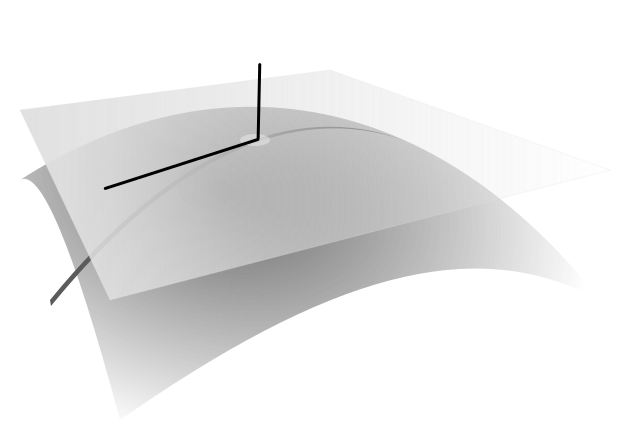
\includegraphics[width=0.8\textwidth]{tangent.pdf}
    \caption{Tangent plane and normal vector}
\end{figure}


\section{Derivatives of vector fields}

Essentially everything discussed above for scalar fields extends to vector fields in a predictable way.
This is because of the linearity and that we can consider each \emph{component} of the vector field independently.

\begin{definition}[directional derivative]
    Let \(S\subset \bR^n\) and \(\ff:S\to \bR^m\).
    For any \(\aa \in \operatorname{int}S\) and \(\vv \in \bR^n\) the derivative of the vector field \(\ff\) with respect to \(\vv\) is defined as
    \[
        D_{\vv}\ff(\aa) :=
        \lim_{h\to 0} \frac{1}{h} \left(\ff(\aa+h \vv) - \ff(\aa)\right).
    \]
\end{definition}

\begin{remark}
    If we use the notation \(\ff = (f_1,\ldots,f_m)\), i.e., we write the function using the ``components'' where each \(f_k\) is a scalar field, then \(D_{\vv}\ff = (D_{\vv}f_1,\ldots,D_{\vv} f_m)\).
\end{remark}


\begin{definition*}[differentiable]
    We say that \(\ff: \bR^n \to \bR^m\) is \emph{differentiable} at \(\aa\) if there exists a linear transformation \({df}_{\aa}: \bR^n \to \bR^m\) such that, for \(\xx \in B(\aa,r)\),
    \[
        \ff(\xx) = \ff(\aa) + {df}_{\aa}(\xx-\aa) + \epsilon(\xx-\aa)
    \]
    \(\abs{\epsilon(\xx-\aa)} = \littleo{\norm{\xx-\aa}}\).
\end{definition*}


\begin{theorem}
    If \(\ff\) is differentiable at \(\aa\)
    then \(\ff\) is continuous at \(\aa\)
    and \( {df}_{\aa}(\vv) =D_{\vv}\ff(\aa) \).
\end{theorem}

\begin{proof}
    Same as for the case of scalar fields when \(f:\bR^n \to \bR\).
\end{proof}


\section{Jacobian matrix and chain rule}

The relevant differential for higher-dimensional functions is the \href{https://en.wikipedia.org/wiki/Jacobian_matrix_and_determinant}{Jacobian matrix}.

\begin{definition}[Jacobian matrix]
    Suppose that \(\ff: \bR^2 \to \bR^2\) and use the notation \(\ff(x,y) = (f_1(x,y),f_2(x,y))\).
    The \emph{Jacobian matrix} of \(\ff\) at \(\aa\) is defined as
    \[
        D\ff(\aa) =
        \begin{pmatrix}
            \frac{\partial f_1}{\partial x} (\aa) & \frac{\partial f_1}{\partial y} (\aa) \\[2pt]
            \frac{\partial f_2}{\partial x} (\aa) & \frac{\partial f_2}{\partial y} (\aa)
        \end{pmatrix}.
    \]
\end{definition}

\begin{remark*}
    The \emph{Jacobian matrix} is defined analogously in any dimension.
    I.e., if \(\ff : \bR^n \to \bR^m\) the the Jacobian at \(\aa\) is
    \[
        D\ff(\aa) =
        \begin{pmatrix}
            \partial_1 f_1 (\aa) & \partial_2 f_1 (\aa) & \cdots & \partial_n f_1 (\aa) \\
            \partial_1 f_2 (\aa) & \partial_2 f_2 (\aa) & \cdots & \partial_n f_2 (\aa) \\
            \vdots               & \vdots               &        & \vdots               \\
            \partial_1 f_m (\aa) & \partial_2 f_m (\aa) & \cdots & \partial_n f_m (\aa)
        \end{pmatrix}
    \]
\end{remark*}


If we choose a basis then any linear transformation \(\bR^n \to \bR^m\) can be written as a \(m \times n\) matrix.
We find that \( {df}_{\aa}(\vv ) = D\ff(\aa) \vv\).

Let \(S\subset \bR^n\) and \(\ff : S \to \bR^m\).
If \(f\) is differentiable at \(\aa \in S\) then, for all  \(\xx\in B(\aa,r) \subset S\),
\[
    \ff(\xx) = \ff(\aa) +  D\ff(\aa) (\xx-\aa) + \epsilon(\xx-\aa)
\]
where \(\abs{\epsilon(\xx-\aa)} = \littleo{\norm{\xx-\aa}}\).
This is like a Taylor expansion in higher dimensions.

Here we see that in higher dimensions we have a matrix form of the chain rule.

\begin{theorem}
    \label{thm:jacobian-chain}
    Let \(S\subset \bR^l\), \(T\subset \bR^m\) be open.
    Let \(\ff: S \to T\) and \(\gg:T \to \bR^n\) and define
    \[
        \hh := \gg \circ \ff : S \to \bR^n.
    \]
    Let  \(\aa\in S\). Suppose that \(\ff\) is differentiable at \(\aa\) and \(\gg\) is differentiable at \(\ff(\aa)\).
    Then \(\hh\) is differentiable at \(\aa\) and
    \[
        D\hh(\aa) = D\gg(\ff(\aa)) \ D\ff(\aa).
    \]
\end{theorem}

\begin{proof}
    Let \(\uu = \ff(\aa+\vv) - \ff(\aa) \).
    Since \(\ff\) and \(\gg\) are differentiable,
    \[
        \begin{aligned}
            \hh(\aa+\vv) - \hh(\aa)
             & = \gg(\ff(\aa+\vv)) - \gg(\ff(\aa))                                                                                    \\
             & = D\gg(\ff(\aa))(\ff(\aa+\vv) - \ff(\aa) ) + \boldsymbol{\epsilon}_{\gg}(\uu)                                          \\
             & = D\gg(\ff(\aa))   D\ff(\aa) \vv + D\gg(\ff(\aa))\boldsymbol{\epsilon}_{\ff}(\vv)  + \boldsymbol{\epsilon}_{\gg}(\uu).
        \end{aligned} \qedhere
    \]
\end{proof}



\begin{example}[polar coordinates]
    Here we consider \emph{polar coordinates} and calculate the Jacobian of this transformation.
    We can write the change of coordinates
    \[
        (r,\theta) \mapsto (r\cos \theta, r\sin \theta)
    \]
    as the function  \(\ff(r,\theta) = (x(r,\theta),y(r,\theta))\) where \(\ff:(0,\infty)\times [0,2\pi) \to \bR^2\).
    We calculate the Jacobian matrix of this transformation
    \[
        D\ff(r,\theta) =
        \begin{pmatrix}
            \tfrac{\partial x}{\partial r}(r,\theta) & \tfrac{\partial x}{\partial \theta}(r,\theta) \\[2pt]
            \tfrac{\partial y}{\partial r}(r,\theta) & \tfrac{\partial y}{\partial \theta}(r,\theta)
        \end{pmatrix}
        =
        \begin{pmatrix}
            \cos \theta & -r\sin \theta \\
            \sin \theta & r\cos \theta
        \end{pmatrix}.
    \]
    In particular we see that \(\det D\ff(r,\theta) = r\), the familiar value used in change of variables with polar coordinated.

    Suppose now that we wish to calculate derivatives of \(h := g \circ \ff\) for some  \(g:\bR^2 \to \bR\).
    Here we take advantage of Theorem~\ref{thm:jacobian-chain}.
    \[
        \begin{aligned}
            Dh(r,\theta) & = Dg(\ff(r,\theta)) \ D\ff(r,\theta) \\
            \begin{pmatrix}
                \frac{\partial h}{\partial r}(r,\theta) & \frac{\partial h}{\partial \theta}(r,\theta)
            \end{pmatrix}
                         & =
            \begin{pmatrix}
                \frac{\partial g}{\partial x}(\ff(r,\theta)) & \frac{\partial g}{\partial y}(\ff(r,\theta))
            \end{pmatrix}
            \begin{pmatrix}
                \cos \theta & -r\sin \theta \\
                \sin \theta & r\cos \theta
            \end{pmatrix}
        \end{aligned}
    \]
    In other words, we have shown that
    \[
        \begin{aligned}
            \frac{\partial h}{\partial r}(r,\theta)
             & = \frac{\partial g}{\partial x}(r\cos \theta, r\sin \theta) \cos \theta + \frac{\partial g}{\partial y}(r\cos \theta, r\sin \theta)\sin \theta         \\
            \frac{\partial h}{\partial \theta}(r,\theta)
             & = - r \frac{\partial g}{\partial x}(r\cos \theta, r\sin \theta) \sin \theta +  r \frac{\partial g}{\partial y}(r\cos \theta, r\sin \theta)\cos \theta.
        \end{aligned}
    \]
\end{example}






\section{Implicit functions and partial derivatives}

Just like with derivatives, we can take higher order partial derivatives.
\begin{remark*}
    For convenience when we want to write \(\frac{\partial}{\partial y}\frac{\partial}{\partial x}f(x,y) \), i.e., differentiate first with respect to \(x\) and then with respect to \(y\), we write instead \(\frac{\partial^2 f}{\partial y \partial x}(x,y) \).
    The analogous notation is used for higher derivatives and any other choice of coordinates.
\end{remark*}

We first consider the question of when
\[
    \frac{\partial^2 f}{\partial y \partial x}(x,y)
    \overset{\text{\large\color{blue} ?}}{=}
    \frac{\partial^2 f}{\partial x \partial y}(x,y).
\]

\begin{example*}[partial derivative problem]
    Let \(f:\bR^2 \to \bR\) be defined as \(f(0,0)=0\) and, for \((x,y)\neq (0,0)\),
    \[
        f(x,y) := \frac{x y(x^2 - y^2)}{x^2 + y^2}.
    \]
    We calculate that \(\frac{\partial^2 f}{\partial y \partial x} (0,0) = -1\) but
    \(\frac{\partial^2 f}{\partial x \partial y}(0,0) = 1\).
\end{example*}

\begin{theorem}
    Let \(f:S\to\bR\) be a scalar field such that the partial derivatives \(\frac{\partial f}{\partial x }\), \(\frac{\partial f}{\partial y}\) and \(\frac{\partial^2 f}{\partial y \partial x} \) exist on an open set \(S\subset \bR^2\) containing \(\xx\).
    Further assume that \(\frac{\partial^2 f}{\partial y \partial x} \) is continuous on \(S\).
    Then the derivative \(\frac{\partial^2 f}{\partial x \partial y} (\xx)\) exists and
    \[
        \frac{\partial^2 f}{\partial x \partial y} (\xx)=\frac{\partial^2 f}{\partial y \partial x} (\xx).
    \]
\end{theorem}

In many cases we can choose to write a given curve/function either in \emph{implicit} or \emph{explicit} form.

\begin{center}
    \begin{tabular}{c | c}
        \textbf{Implicit}         & \textbf{Explicit}                              \\
        \hline
        \(x^2-y=0\)               & \(y(x) = x^2\)                                 \\
        \(x^2+y^2=1\)             & \(y(x) = \pm \sqrt{1-x^2}\), \(\abs{x}\leq 1\) \\
        \(x^2-y^2-1=0\)           & \(y(x) = \pm \sqrt{x^2-1}\), \(\abs{x}\geq 1\) \\
        \(x^2+y^2-e^y -4 =0\)     & A mess?                                        \\
        \(x^2y^4 - 3 = \sin(xy)\) & A huge mess?
    \end{tabular}
\end{center}

Given the above observation, the following method of calculating derivatives is sometimes useful.
Suppose that some \(f:\bR^2 \to \bR\) is given and we suppose there exists some \(y:\bR\to\bR\) such that
\[
    f(x,y(x))=0 \quad \text{ for all \(x\)}.
\]
Let \(h(x):= f(x,y(x))\) and note that \(h'(x)=0\).
Here we are using the idea that \(h = f \circ g\) where \(g(x) = (x,y(x))\).
By the chain rule \( h'(x)\) is equal to
\[
    \begin{pmatrix}
        \frac{\partial f}{\partial x}(x,y(x)) & \frac{\partial f}{\partial y}(x,y(x))
    \end{pmatrix}
    \begin{pmatrix}
        1 \\
        y'(x)
    \end{pmatrix}
    =0.
\]
Consequently
\[
    y'(x) = - \frac{ \frac{\partial f}{\partial x}(x,y(x)) }{ \frac{\partial f}{\partial y}(x,y(x)) }.
\]

% !TeX root = ../main.tex
\chapter{Extrema \& other applications}

\lettrine{I}{n} the previous chapter we introduced various notions of differentials for higher dimensional functions (scalar fields, vector fields, paths, etc.).
In this chapter we now explore various applications of these notions and work with some of the implementations, rather than just the objects.
Firstly we will consider certain partial differential equations which we now have the tools to solve.
Then the majority of the chapter is devoted to searching for extrema (minima / maxima) in various different scenarios.
This extends what we already know for functions in \(\bR\) and we will find that in higher dimensions many more possibilities and subtleties exist.

\section{Partial differential equations}

There are a huge number of different types of partial differential equations (PDEs) and here we consider just two types, \emph{first order linear PDEs} and the \emph{1D wave equation}.
We start by consider an example of the first type.

\begin{example*}
    Find all solutions of the PDE
    \(3 \frac{\partial f}{\partial x}(x,y) + 2 \frac{\partial f}{\partial y} (x,y) = 0\).
\end{example*}

\begin{solution}
    The given PDE is equivalent to
    \(\left( \begin{smallmatrix}
            3 \\ 2
        \end{smallmatrix} \right)
    \cdot
    \nabla f(x,y) =0\).
    We can also phrase this in terms of the directional derivative, namely
    \[
        D_{v}f(x,y) = 0 \quad \text{where \(v=\left( \begin{smallmatrix}
                3 \\ 2
            \end{smallmatrix} \right)\)}.
    \]
    This means that if a function \(f\) is a solution to the PDE then it is constant in the direction \(\left( \begin{smallmatrix}
            3 \\ 2
        \end{smallmatrix} \right)\).
    This means that all solutions have the form \(f(x,y) = g(2x-3y)\) for some \(g:\bR \to \bR\).
\end{solution}

The same idea as used for the above example gives the following general result.

\begin{theorem}
    Let \(g:\bR\to\bR\) be differentiable, \(a,b\in \bR\), \((a,b)\neq (0,0)\).
    If \(f(x,y)= g(bx-ay)\) then
    \[
        a \frac{\partial f}{\partial x} (x,y) + b \frac{\partial f}{\partial y} (x,y) = 0.
    \]
    Conversely, every \(f\) which satisfies this equation is of the form \(g(bx-ay)\).
\end{theorem}

\begin{proof}
    First we prove \textbf{(\(\boldsymbol\Rightarrow\))}.
    If \(f(x,y)= g(bx-ay)\) then, by the chain rule,
    \[
        \partial_x f(x,y) = bg'(bx-ay),
        \quad
        \partial_y f(x,y) = -ag'(bx-ay).
    \]
    Consequently \(a\partial_x f(x,y) + b \partial_y f(x,y) = a bg'(bx-ay) - abg'(bx-ay) = 0\).
    Now we prove \textbf{(\(\boldsymbol\Leftarrow\))}.
    It's convenient to work in coordinates which correspond to the lines along which the solutions are constant.
    Let \(\left(\begin{smallmatrix}
            u\\ v
        \end{smallmatrix}\right)
    = \left(\begin{smallmatrix}
            a & b \\ b & -a
        \end{smallmatrix}\right)
    \left(\begin{smallmatrix}
            x \\ y
        \end{smallmatrix}\right)\).
    This means that
    \(\left(\begin{smallmatrix}
            x\\ y
        \end{smallmatrix}\right)
    = \frac{-1}{a^2 + b^2} \left(\begin{smallmatrix}
            a & b \\ b & -a
        \end{smallmatrix}\right)
    \left(\begin{smallmatrix}
            u \\ v
        \end{smallmatrix}\right)\).
    Let \(h(u,v)=f(\frac{au + bv}{a^2 + b^2}, \frac{bu-av}{a^2+b^2})\).
    We calculate that
    \[
        \partial_u h(u,v)
        = \tfrac{1}{{a^2 + b^2}}
        \left( a \partial_x f
        + b \partial_y f \right)  (au + bv, bu-av) = 0.
    \]
    Namely, \(h(u,v)\) is a function of \(v\) only so take \(g(v) = h(u,v)\) and so \(f(x,y) = g(bx-ay)\).
\end{proof}

Now we look at another type of PDE.
The \href{https://en.wikipedia.org/wiki/Wave_equation}{\emph{1D wave equation}} is
\[
    \frac{\partial^2 f}{\partial x^2}(x,t) = c^2  \frac{\partial^2 f}{\partial t^2}(x,t).
\]
Here \(x\) represents the position along string,
\(t\) is time and \(f(x,t)\) is the displacement of the string from the centre at position \(x\), at time \(t\).
The constant \(c\) is a fixed parameter depending on the string.

This partial differential equation is derived from the equation of motion \(F = m a\) where \(F\) is the tension in the string, \(a\) is the acceleration from horizontal and \(m\) is the mass of a little piece of the string.
The equation is valid for small displacement.
In this case the \emph{boundary conditions} are natural: Are the ends of the string fixed? Is only one end fixed? At time \(t=0\), is the string already moving?

\begin{theorem}
    Let \(F\) be a twice differentiable function and \(G\) a differentiable function.

    \noindent
    \textbf{1.} The function defined as
    \begin{equation}
        \label{eq:wave}
        f(x,t) = \frac{1}{2}(F(x+ct) + F(x-ct)) + \frac{1}{2c} \int_{x-ct}^{x+ct} G(s) \ ds
    \end{equation}
    satisfies \(   \frac{\partial^2 f}{\partial x^2}(x,t) = c^2  \frac{\partial^2 f}{\partial t^2}(x,t) \),
    \(f(x,0) = F(x)\)
    and \(\frac{\partial f}{\partial t}(x,0) = G(x)\).

    \noindent
    \textbf{2.} Conversely, if a solution of
    \[
        \frac{\partial^2 f}{\partial x^2}(x,t) = c^2  \frac{\partial^2 f}{\partial t^2}(x,t)
    \]
    satisfies
    \(\frac{\partial^2 f}{\partial x \partial t} = \frac{\partial^2 f}{\partial t \partial x}\),
    then it has the above form \eqref{eq:wave}.
\end{theorem}


\begin{proof}[Proof of part 1.]
    Let \(f(x,t)\) be as defined \eqref{eq:wave} in the statement of the theorem.
    We calculate the partial derivatives
    \[
        \begin{aligned}
            \tfrac{\partial f}{\partial x} (x,t)
             & = \tfrac{1}{2} \left(F'(x+ct) + F'(x-ct)\right)          \\
             & \quad\quad\quad
            + \tfrac{1}{2c}\left(G(x+ct) - G(x-ct)\right)               \\
            \tfrac{\partial^2 f}{\partial x^2}(x,t)
             & = \tfrac{1}{2} \left(F''(x+ct) + F''(x-ct)\right)        \\
             & \quad\quad\quad
            + \tfrac{1}{2c}\left(G'(x+ct) - G'(x-ct)\right)             \\
            \tfrac{\partial f}{\partial t} (x,t)
             & = \tfrac{1}{2} \left(cF'(x+ct) - c F'(x-ct)\right)       \\
             & \quad\quad\quad
            + \tfrac{1}{2}\left(G(x+ct) + G(x-ct)\right)                \\
            \tfrac{\partial^2 f}{\partial t^2} f(x,t)
             & = \tfrac{1}{2} \left(c^2F''(x+ct) + c^2 F''(x-ct)\right) \\
             & \quad\quad\quad
            + \tfrac{c}{2}\left(G'(x+ct) + G'(x-ct)\right).
        \end{aligned}
    \]
    From this calculation we see that  \(   \frac{\partial^2 f}{\partial x^2}(x,t) = c^2  \frac{\partial^2 f}{\partial t^2}(x,t) \).
    Additionally \(f(x,0) = F(x)\)
    and \(\frac{\partial f}{\partial t}(x,0) = G(x)\).
\end{proof}

\begin{proof}[Proof of part 2.]
    Suppose that \(f\) satisfies the 1D wave equation;
    Introduce \(u = x + ct\), \(v=x-ct\)
    and observe that \(x = \frac{u+v}{2}\), \(t=\frac{u-v}{2c}\).
    Define \(g(u,v) = f(   \frac{u+v}{2} , \frac{u-v}{2c} )\).
    By the chain rule
    \[
        \begin{aligned}
            \tfrac{\partial g}{\partial u}(u,v)
             & = \tfrac{1}{2} \tfrac{\partial f}{\partial x}(   \tfrac{u+v}{2} , \tfrac{u-v}{2c} )
            + \tfrac{1}{2c} \tfrac{\partial f}{\partial t}(   \tfrac{u+v}{2} , \tfrac{u-v}{2c} ),                     \\
            \tfrac{\partial^2 g}{\partial v \partial u}(u,v)
             & = \tfrac{1}{4} \tfrac{\partial^2 f}{\partial x^2}(   \tfrac{u+v}{2} , \tfrac{u-v}{2c} )
            - \tfrac{1}{4c} \tfrac{\partial^2 f}{\partial x\partial t}(   \tfrac{u+v}{2} , \tfrac{u-v}{2c} )          \\
             & \ \ +  \tfrac{1}{4c} \tfrac{\partial^2 f}{\partial x \partial t}(   \tfrac{u+v}{2} , \tfrac{u-v}{2c} )
            -  \tfrac{1}{4c^2} \tfrac{\partial^2 f}{\partial t^2}(   \tfrac{u+v}{2} , \tfrac{u-v}{2c} ) = 0.
        \end{aligned}
    \]
    Since the second derivative is zero we know that \(\tfrac{\partial g}{\partial u}\) is constant in \(v\), therefore we can write \( \tfrac{\partial g}{\partial u}(u,v) = \varphi_0(u)\).
    In turn this means we can write \(g(u,v) = \varphi_1(u) + \varphi_2(v)\).
    I.e., \(f(x,t) = \varphi_1(x+ct) + \varphi_2(x-ct)\).
    Let
    \[
        F(x) = \varphi_1(x) + \varphi_2(x).
    \]
    This means that
    \(F'(x) = \varphi_1'(x) + \varphi_2'(x)\)
    and \(\frac{\partial f}{\partial t}(x,t) = c\varphi_1(x+ct) - c\varphi_2(x-ct)\).
    Let
    \[
        G(x) = \tfrac{\partial f}{\partial t}(x,0) = c\varphi_1(x) - c\varphi_2(x). \qedhere
    \]
    Substituting these quantities we show that the required form~\eqref{eq:wave} is satisfied.
\end{proof}

\section{Extrema (minima / maxima / saddle)}

Let \(S\subset \bR^n\) be open,
\(f:S \to \bR\) be a scalar field
and \(\aa \in S\).

\begin{definition}[absolute min/max]
    If \(f(\aa)\leq f(\xx)\) (resp.\ \(f(\aa)\geq f(\xx)\)) for all \(\xx \in S\), then \(f(\aa)\) is said to be the \emph{absolute} minimum (resp.\ maximum) of \(f\).
\end{definition}

\begin{definition}[relative min/max]
    If \(f(\aa)\leq f(\xx)\) (resp.\ \(f(\aa)\geq f(\xx)\)) for all \(\xx \in B(\aa,r)\) for some \(r>0\), then \(f(\aa)\) is said to be a \emph{relative} minimum (resp.\ maximum) of \(f\).
\end{definition}

Collectively we call the these points the \emph{extrema} of the scalar field.
In the case of a scalar field defined on \(\bR^2\) we can visualize the scalar field as a 3D plot like Figure~\ref{fig:bumps}.
Here we see the extrema as the ``flat'' places.
We sometimes use \emph{global} as a synonym of \emph{absolute} and \emph{local} as a synonym of \emph{relative}.


\begin{figure}[htbp]
    \begin{center}
        \includegraphics{bumps.pdf}
        \caption{$f(x,y) := x e^{-(x^2y^2)}  + \frac{1}{4}e^{y^\frac{3}{10}}$}
        \label{fig:bumps}
    \end{center}
\end{figure}

To proceed it is convenient to connect the extrema with the behaviour of the gradient of the scalar field.

\begin{theorem}
    \label{thm:is-stationary}
    If \(f:S\to\bR\) is differentiable and has a relative minimum or maximum at \(\aa\), then \(\nabla f(\aa)=  \mathbf{0}\).
\end{theorem}

\begin{proof}
    Suppose \(f\) has a relative minimum at \(\aa\) (or consider \(-f\)).
    For any unit vector \(\vv\) let \(g(u) = f(\aa+u\vv)\).
    We know that \(g:\bR \to \bR\) has a relative minimum at \(u=0\) so \(u'(0)=0\).
    This means that the directional derivative \(D_{\vv} f(\aa) = 0\) for every \(\vv\).
    Consequently this means that \(\nabla f (\aa)= \mathbf{0}\).
\end{proof}

\begin{figure}[htbp]
    \begin{center}
        \includegraphics[width=0.5\textwidth]{inflection.pdf}
        \caption{\(\nabla f(\aa) =  \mathbf{0}\) doesn't imply a minimum or maximum at \(\aa\), even in \(\bR\), as seen with the function \(f(x):=x^3\). In higher dimensions even more is possible.}
        \label{fig:inflection}
    \end{center}
\end{figure}

Observe that here and in the subsequent text, we can always consider the case of \(f:\bR \to \bR\), i.e., the case of \(\bR^n\) where \(n=1\).
Everything still holds and reduces to the arguments and formulae previously developed for functions of one variable.


\begin{definition}[stationary point]
    If \(\nabla f(\aa)=\mathbf{0}\) then \(\aa\) is called a \emph{stationary point}.
\end{definition}


\begin{figure}[htbp]
    \begin{center}
        \includegraphics[width=0.5\textwidth]{bowl.pdf}
        \caption{If \(f(x,y)=x^2+y^2\) then \(\nabla f(x,y) = \left(\begin{smallmatrix}
                2x\\2y
            \end{smallmatrix}\right)\) and \(\nabla f(0,0) =\left(\begin{smallmatrix}
                0\\0
            \end{smallmatrix}\right) \). The point \((0,0)\) is an absolute minimum for \(f\).}
    \end{center}
\end{figure}

As we see in the example of Figure~\ref{fig:inflection}, the converse of Theorem~\ref{thm:is-stationary} fails in the sense that a stationary point might not be a minimum or a maximum.
The motivates the following.

\begin{definition}[saddle point]
    If \(\nabla f(\aa)=\mathbf{0}\) and \(\aa\) is neither a minimum nor a maximum then \(\aa\) is said to be a \emph{saddle point}.
\end{definition}

The quintessential saddle has the shape seen in Figure~\ref{fig:pringle}.
However it might be similar to Figure~\ref{fig:inflection} or more complicated using the possibilities available in higher dimension.

\begin{figure}[htbp]
    \centering
    \includegraphics{pringle.pdf}
    \caption{If \(f(x,y)=x^2-y^2\) then \(\nabla f(x,y) = \left(\begin{smallmatrix}
            2x\\-2y
        \end{smallmatrix}\right)\) and \(\nabla f(0,0) =\left(\begin{smallmatrix}
            0\\0
        \end{smallmatrix}\right) \). The point \((0,0)\) is a saddle point for \(f\).}
    \label{fig:pringle}
\end{figure}


\section{Hessian matrix}

To proceed it is useful to develop the idea of a second order Taylor expansion in this higher dimensional setting.
In particular this will allow us to identify the local behaviour close to stationary points.
The main object for doing this is the \emph{Hessian matrix}.

\begin{definition}[Hessian matrix]
    Let \(f:\bR^2 \to\bR\) be twice differentiable and use the notation \(f(x,y)\).
    The \emph{Hessian matrix} at \(\aa\in \bR^2\) is defined as
    \[
        \mathbf{H} f (\aa)= \begin{pmatrix}
            \dfrac{\partial^2 f}{\partial x^2} (\aa)
             & \dfrac{\partial^2 f}{\partial x\,\partial y} (\aa)
            \\[2.2ex]
            \dfrac{\partial^2 f}{\partial y\,\partial x} (\aa)
             & \dfrac{\partial^2 f}{\partial y^2}(\aa)
        \end{pmatrix}.
    \]
\end{definition}

Observe that the Hessian matrix \(\mathbf{H} f (\aa)\) is a symmetric matrix since we know that \(\frac{\partial^2 f}{\partial x\,\partial y} (\aa) = \frac{\partial^2 f}{\partial y\,\partial x} (\aa)\) for twice differentiable functions (Theorem~\ref{thm:equal-double-partial}).
The Hessian matrix is defined analogously in any dimensions as follows.
Let \(f:\bR^n \to\bR\) be twice differentiable.
The \emph{Hessian matrix} at \(\aa\in \bR^n\) is defined as
\[
    \mathbf{H} f (\aa)= \begin{pmatrix}
        \dfrac{\partial^2 f}{\partial x_1^2} (\aa)
         & \dfrac{\partial^2 f}{\partial x_1\,\partial x_2} (\aa)
         & \cdots
         & \dfrac{\partial^2 f}{\partial x_1\,\partial x_n}(\aa)  \\[2.2ex]
        \dfrac{\partial^2 f}{\partial x_2\,\partial x_1} (\aa)
         & \dfrac{\partial^2 f}{\partial x_2^2}(\aa)
         & \cdots
         & \dfrac{\partial^2 f}{\partial x_2\,\partial x_n}(\aa)  \\[2.2ex]
        \vdots
         & \vdots
         & \ddots
         & \vdots                                                 \\[2.2ex]
        \dfrac{\partial^2 f}{\partial x_n\,\partial x_1} (\aa)
         & \dfrac{\partial^2 f}{\partial x_n\,\partial x_2} (\aa)
         & \cdots
         & \dfrac{\partial^2 f}{\partial x_n^2}(\aa)
    \end{pmatrix}.
\]

Observe that the Hessian matrix is a real symmetric matrix in any dimension.
If \(f:\bR \to \bR\) then \(\mathbf{H} f (a)\) is a \(1\times 1\) matrix and coincides with the second derivative of \(f\).
In this sense what we know about extrema in \(\bR\) is just a special case of everything we do here.

\begin{lemma*}
    If \(\vv= \left( \begin{smallmatrix}
            v_1\\ \vdots \\v_n
        \end{smallmatrix} \right)  \) then\footnote{The notation \(\vv^{\mathbf{t}}\) denotes the transpose of the vector \(\vv\).} \(\vv^{\mathbf{t}} \ \mathbf{H} f (\aa) \ \vv = \sum_{j,k=0}^{n}
    \partial_{j}\partial_{k}f(\aa)
    v_j v_k \in \bR\).
\end{lemma*}

\begin{proof}
    Multiplying the matrices we calculate that\footnote{For convenience, here and in many other places of this text, we use the notation
        \(\partial_{j}\partial_{k}f(\aa) = \frac{\partial^2 f}{\partial x_j\,\partial x_k} (\aa)\).}
    \[
        \begin{aligned}
            \vv^{\mathbf{t}} \ \mathbf{H} f (\aa) \ \vv
             & =
            \begin{pmatrix}
                v_1 & \cdots & v_n
            \end{pmatrix}
            \begin{pmatrix}
                \partial_{1}\partial_{1}f(\aa) & \cdots &
                \partial_{1}\partial_{n}f(\aa)                   \\
                \vdots                         & \ddots & \vdots \\
                \partial_{n}\partial_{1}f(\aa) & \cdots &
                \partial_{n}\partial_{n}f(\aa)
            \end{pmatrix}
            \begin{pmatrix}
                v_1 \\ \vdots \\v_n
            \end{pmatrix} \\
             & = \sum_{j,k=0}^{n}
            \partial_{j}\partial_{k}f(\aa)
            v_j v_k
        \end{aligned}
    \]
    as required.
\end{proof}


\begin{example*}
    Let \(f(x,y)=x^2-y^2\) (Figure~\ref{fig:pringle}).
    The gradient and the Hessian are respectively
    \[
        \begin{aligned}
            \nabla f(x,y)      & =\begin{pmatrix}
                \frac{\partial f}{\partial x} (x,y) \\[2pt]
                \frac{\partial f}{\partial y} (x,y)
            \end{pmatrix} =   \begin{pmatrix}
                2x \\-2y
            \end{pmatrix}, \\
            \mathbf{H} f (x,y) & = \begin{pmatrix}
                \frac{\partial^2 f}{\partial x^2} (x,y)
                 & \frac{\partial^2 f}{\partial x\,\partial y} (x,y)
                \\[2pt]
                \frac{\partial^2 f}{\partial y\,\partial x} (x,y)
                 & \frac{\partial^2 f}{\partial y^2}(x,y)
            \end{pmatrix}
            = \begin{pmatrix}
                2
                 & 0
                \\[2.2ex]
                0
                 & -2
            \end{pmatrix}.
        \end{aligned}
    \]
    The point \((0,0)\) is a stationary point since \(\nabla f(0,0) =\left(\begin{smallmatrix}
            0\\0
        \end{smallmatrix}\right) \).
    In this example \(\mathbf{H} f \) does not depend on \((x,y)\) but in general we can expect dependence and so it gives a different matrix at different points  \((x,y)\).
\end{example*}


\subsubsection*{Second order Taylor formula for scalar fields}

First let's recall the first order Taylor approximation from Theorem~\ref{thm:differential}.
If \(f\) is differentiable at \(\aa\)
then
\(  f(\xx) \approx f(\aa)  + \nabla f(\aa) \cdot (\xx-\aa)\).
If \(\aa\) is a stationary point then this only tells us that \(  f(\xx) \approx f(\aa) \) so a natural next question is to search for slightly more detailed information.

\begin{theorem}[second order Taylor]
    Let \(f\) be a scalar field twice differentiable on \(B(\aa,r)\).
    Then,\footnote{We use the convention that \((\xx-\aa)\) is a vertical vector, equivalently, a \(n \times 1\) matrix.} for \(\xx\) close to \(\aa\),
    \[
        f(\xx) \approx f(\aa) + \nabla f(\aa) \cdot (\xx-\aa) + \frac{1}{2} (\xx-\aa)^{\mathbf{t}} \ \mathbf{H} f (\aa) \ (\xx-\aa)
    \]
    in the sense that the error is \(\littleo{\norm{(\xx-\aa)}^2}\).
\end{theorem}

\begin{proof}[Proof of second order Taylor formula]
    Let \(\vv = \xx-\aa\) and let \(g(u) = f(\aa + u \vv)\).
    The Taylor expansion of \(g\) tells us that
    \(g(1) = g(0) + g'(0) + \frac{1}{2} g''(c)\) for some \(c\in (0,1)\).
    Since \(g(u) = f(a_1 + uv_1, \ldots, a_n + u v_n)\), by the chain rule,
    \[
        \begin{aligned}
            g'(u)  & = \sum_{j=1}^{n} \partial_j f( a_1 + uv_1, \ldots, a_n + u v_n ) v_j
            =\nabla f( \aa + u \vv) \cdot \vv,                                                            \\
            g''(u) & = \sum_{j,k=1}^{n} \partial_j\partial_k f( a_1 + uv_1, \ldots, a_n + u v_n ) v_j v_k \\
                   & \quad \quad \quad
            =  \vv^{\mathbf{t}} \ \mathbf{H} f (\aa + u \vv) \ \vv.
        \end{aligned}
    \]
    Consequently
    \(
    f(\aa+\vv) = f(\aa) + \nabla f(\aa) \cdot \vv + \frac{1}{2} \vv^{\mathbf{t}} \ \mathbf{H} f (\aa + c\vv) \ \vv
    \).
    We define the ``error'' in the approximation as \(\epsilon(\vv) = \frac{1}{2}  \vv^{\mathbf{t}} (\mathbf{H} f (\aa + c\vv) - \mathbf{H} f (\aa)  ) \vv\)
    and estimate that
    \[
        \abs{\epsilon(\vv)} \leq \sum_{j,k=0}^{n}
        v_j v_k \left( \partial_{j}\partial_{k}f(\aa+c\vv)-\partial_{j}\partial_{k}f(\aa) \right).
    \]
    Since \(\abs{ v_j v_k} \leq \norm{\vv}^2\) we observe that \(\frac{\abs{\epsilon(\vv)} }{\norm{\vv}^2} \to 0\) as \(\norm{\vv} \to 0\) as required.
\end{proof}


\section{Classifying stationary points}

In order to classify the stationary points we will take advantage of the Hessian matrix and therefore we need to first understand the follow fact about real symmetric matrices.

\begin{theorem}
    Let \(A\) be a real symmetric matrix and let
    \(Q(\vv) =  \vv^{\mathbf{t}} A  \vv  \).
    Then
    \[
        \begin{aligned}
            \text{\(Q(\vv) > 0\) for all \(\vv \neq \mathbf{0}\)}
             & \quad \Longleftrightarrow \quad 
            \text{all eigenvalues of \(A\) are positive}, \\
            \text{\(Q(\vv) < 0\) for all \(\vv \neq \mathbf{0}\)}
             & \quad \Longleftrightarrow \quad
            \text{all eigenvalues of \(A\) are negative}.
        \end{aligned}
    \]
\end{theorem}

\begin{proof}
    Since \(A\) is symmetric it can be diagonalised by  matrix \(B\)  which is orthogonal (\(B^{\mathbf{t}}=B^{-1}\))
    and the diagonal matrix \(D = B^{\mathbf{t}} A B\) has the eigenvalues of \(A\) as the diagonal.
    This means that
    \(Q(\vv) = \vv^{\mathbf{t}} B^{\mathbf{t}} B A B^{\mathbf{t}} B \vv = \ww^{\mathbf{t}} D \ww \)
    where \(\ww = B \vv\).
    Consequently \(Q(\vv) =  \sum_{j} \lambda_j w_j^2\).
    Observe that, if all \(\lambda_j >0\) then \( \sum_{j} \lambda_j w_j^2  >0\).

    In order to prove the other direction in the ``if and only if'' statement, observe that \(Q(B \uu_k ) = \lambda_k\). This means that, if \(Q(\vv) > 0\) for all \(\vv \neq \mathbf{0}\) then \(\lambda_k>0\) for all \(k\).
\end{proof}

\begin{theorem}[classification of stationary points]
    Let \(f\) be a scalar field twice differentiable on \(B(\aa,r)\).
    Suppose  \(\nabla f(\aa) = \mathbf{0}\) and consider the eigenvalues of  \(\mathbf{H} f (\aa)\). 
    Then
    \[
        \begin{aligned}
            \text{{All} eigenvalues are positive}
             & \quad \Longrightarrow \quad 
            \text{relative minimum at \(\aa\)}, \\
            \text{{All} eigenvalues are negative}
             & \quad \Longrightarrow \quad 
            \text{relative maximum at \(\aa\)}, \\
            \text{Some positive, some negative}
             & \quad \Longrightarrow \quad 
            \text{\(\aa\) is a saddle point}.
        \end{aligned}
    \]
\end{theorem}

\begin{proof}
    Let \(Q(\vv) =  \vv^{\mathbf{t}} \mathbf{H} f (\aa) \vv  \),  \(\ww = B \vv\) and let \(\Lambda := \min_j \lambda_j\).
    Observe that \(\norm{\ww} =  \norm{\vv}\) and that \(Q(\vv)=  \sum_{j} \lambda_j w_j^2  \geq \Lambda \sum_{j} w_j^2 = \Lambda  \norm{\vv}^2 \).
    We have them 2\textsuperscript{nd}-order Taylor
    \[
        \begin{aligned}
                   f(\aa+\vv) - f(\aa)
        &=  \frac{1}{2} \vv^{\mathbf{t}} \ \mathbf{H} f (\aa) \ \vv +  \epsilon(\vv)\\
        &\geq  \left(\tfrac{\Lambda}{2} - \tfrac{\epsilon(\vv)}{\norm{\vv}^2} \right) \norm{\vv}^2.
        \end{aligned}
    \]
    Since \(\frac{\abs{\epsilon(\vv)}}{\norm{\vv}^2} \to 0\) as \(\norm{\vv}\to 0\), \( \frac{\abs{\epsilon(\vv)}}{\norm{\vv}^2} < \tfrac{\Lambda}{2}\) when \(\norm{\vv}\) is small.
    The argument is analogous for the second part. For final part consider \(\vv_j\) which is the eigenvector for \(\lambda_j\) and apply the argument of the first or second part.
\end{proof}

\section{Attaining extreme values}

Here we explore the extreme value theorem for continuous scalar fields.
The argument will be in two parts:
Firstly we show that continuity implies boundedness;
Secondly we show that boundedness implies that the maximum and minimum are attained.
We use the following notation for \emph{intervals} / \emph{rectangles} / \emph{cuboids} / \emph{tesseracts}, etc.
If \(\aa = (a_1,\ldots,a_n)\) and  \(\bb = (b_1,\ldots,b_n)\)
then we consider the \(n\)-dimensional closed Cartesian product
\[
    [\aa,\bb] = [a_1,b_1] \times \cdots \times [a_n,b_n].
\]
We call this set a \emph{rectangle} (independent of the dimension).
As a first step it is convenient to know that all sequences in our setting have convergent subsequences.

\begin{theorem}[Bolzano–Weierstrass]
    If \({\{\xx_{n}\}}_{n}\) is a sequence in \( [\aa,\bb]\)
    there exists a convergent subsequence \({\{\xx_{n_j}\}}_{j}\).
\end{theorem}

\begin{proof}
    In order to prove the theorem we construct the subsequence.
    Firstly we divide \( [\aa,\bb]\) into sub-rectangles of size half the original.
    We then choose a sub-rectangle which contains infinite elements of the sequence and choose the first of these elements to be part of the sub-sequence.
    We repeat this process by again dividing the sub-rectangle we chose by half and choosing the next element of the subsequence.
    We repeat to give the full subsequence.
\end{proof}

\begin{theorem}[boundedness of continuous scalar fields]
    Suppose that \(f\) is a scalar field continuous at every point in the closed rectangle \([\aa,\bb]\).
    Then \(f\) is bounded on \([\aa,\bb]\) in the sense that there exists \(C>0\) such that \(\abs{f(\xx)} \leq C\) for all \(\xx \in [\aa,\bb]\).
\end{theorem}

\begin{proof}
    Suppose the contrary: for all \(n\in\bN\) there exists \(\xx_n\in [\aa,\bb]\) such that \(\abs{f(\xx_n)}>n\).
    \href{https://en.wikipedia.org/wiki/Bolzano%E2%80%93Weierstrass_theorem}{Bolzano–Weierstrass} theorem means that there exists a subsequence \({\{\xx_{n_j}\}}_{j}\) converges to \( \xx \in [\aa,\bb]\).
    Continuity of \(f\) means that \(f(\xx_{n_j})\) converges to \(f(\xx)\). This is a contradiction and hence the theorem is proved.
\end{proof}


We can now use the above result on the boundedness in order to show that the  extreme values are actually obtained.

\begin{theorem}[extreme value theorem]
    Suppose that \(f\) is a scalar field continuous at every point in the closed rectangle \([\aa,\bb]\).
    There there exist points \( \xx, \yy \in [\aa,\bb]\) such that
    \[
        f(\xx) = \inf f
        \quad \text{and} \quad
        f(\yy)= \sup f.
    \]
\end{theorem}

\begin{proof}
    By the boundedness theorem \(\sup f\) is finite and so there exists a sequence  \({\{\xx_{n}\}}_{n}\)  such that \(f(\xx_n)\) converges to \(\sup f\).
    Bolzano–Weierstrass theorem implies that there exists a subsequence  \({\{\xx_{n_j}\}}_{j}\) which converges to \( \xx \in [\aa,\bb]\).
    By continuity \(f(\xx_n) \to f(\xx) = \sup f\).
\end{proof}




\section{Extrema with constraints (Lagrange multipliers)}

We now consider a slightly different problem to the one earlier in this chapter.
There we wished to find the extrema of a given scalar field.
Here the general problem is to minimise or maximise a given scalar field \(f(x,y)\) under the constraint \(g(x,y) = 0\).
Subsequently we will also consider the same problem but in higher dimensions.
We can visualize this problem as shown in Figure~\ref{fig:lagrange}.
For this graphic representation we draw the constraint and also various level sets of the function that we want to find the extrema of.
The graphical representation suggests to us that at the ``touching point'' the gradient vectors are parallel.
In other words, \(\nabla f = \lambda \nabla g\) for some \(\lambda \in \bR\).
The implementation of this idea is the \href{https://en.wikipedia.org/wiki/Lagrange_multiplier}{method of Lagrange multipliers}.


\begin{theorem}[Lagrange multipliers]
    Suppose that a differentiable scalar field \(f(x,y)\) has a relative minimum or maximum when it is subject to the constraint
    \[
        g(x,y) = 0.
    \]
    Then there exists a scalar \(\lambda\) such that, at the extremum point,
    \[
        \nabla f = \lambda \nabla g.
    \]
\end{theorem}

In higher dimensions and possibly with additional constraints we have the following general theorem.

\begin{theorem*}[Lagrange multipliers]
    Suppose that a differentiable scalar field \(f(x_1,\ldots,x_n)\) has an relative extrema when it is subject to \(m\) constraints
    \[
        g_1(x_1,\ldots,x_n) = 0,
        \dots , g_m(x_1,\ldots,x_n)=0,
    \]
    where \(m<n\), and the \(\nabla g_k\) are all linearly independent.
    Then there exist \(m\) scalars \(\lambda_1,\ldots,\lambda_m\) such that, at each extremum point,
    \[
        \nabla f = \lambda_1 \nabla g_1 + \cdots + \lambda_m \nabla g_m.
    \]
\end{theorem*}

\begin{figure}[htb]
    \begin{center}
        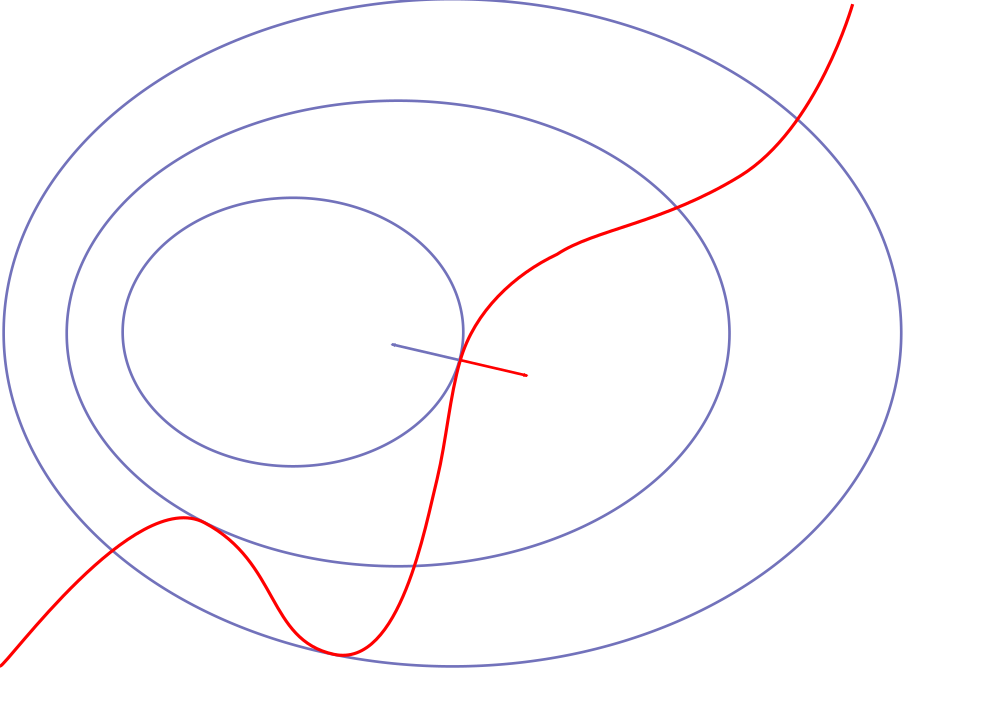
\includegraphics{lagrange.pdf}
        \caption{Searching extrema of \(f\) under constraint \(g=0\)}
        \label{fig:lagrange}
    \end{center}
\end{figure}

The Lagrange multiplier method is often stated and far less often proved. 
Since the proof is rather involved we will follow this tradition here.
See, for example, Chapter 14 of  ``A First Course in Real Analysis''  (2012) by Protter \& Morrey for a complete proof and further discussion.

Let us consider a particular case of the method when \(n=3\) and \(m=2\).
More precisely we consider the following problem: 
Find the maxima and minima of \(f(x,y,z)\) along the curve \(C\) defined as 
\[
    g_1(x,y,z) = 0, 
    \quad
    g_2(x,y,z) = 0
\]
where \(g_1\), \(g_2\) are differentiable functions.
In this particular case we will prove the Lagrange multiplier method.
Suppose that \(\aa\) is some point in the curve.
Let \(\aalpha(t)\) denote a path which lies in the curve \(C\) in the sense that \(\aalpha(t) \in C\) for all \(t\in (-1,1)\), \(\aalpha'(t)\neq \mathbf{0}\) and \(\aalpha(0)=\aa\).
If \(\aa\) is a local minimum for \(f\) restricted to \(C\) it means that \(f(\aalpha(t))\geq f(\aalpha(0))\) for all \(t \in (-\delta,\delta)\) for some \(\delta>0\). 
In words, moving away from \(\aa\) along the curve \(C\) doesn't cause \(f(\xx)\) to decrease.
Let \(h(t) = f(\aalpha(t))\) and observe that \(h:\bR \to \bR\) so we know how to find the extrema.
In particular we know that \(h'(0)=0\).
By the chain rule \(h'(t) = \nabla f(\aalpha(t))\cdot \aalpha'(t)\) and so 
\[
    \nabla f(\aa)\cdot \aalpha'(0) = 0.
\]
Since we know that \(g_1(\aalpha(t))=0\) and \(g_2(\aalpha(t))=0\), again by the chain rule,
\[
    \nabla g_1(\aa)\cdot \aalpha'(0) = 0,
    \quad 
    \nabla g_2(\aa)\cdot \aalpha'(0) = 0.
\]
To proceed it is convenient to isolate the following result of linear algebra.
\begin{lemma*}
    Consider \(w, u_1,u_2 \in \bR^3\) and let \(V = \{v : u_k \cdot v = 0, k =1,2\}\).
    If \(w\cdot v =0\) for all \(v \in V\) then \(w = \lambda_1 u_1 + \lambda_2 u_2\) for some \(\lambda_1,\lambda_2 \in \bR\). 
\end{lemma*}
\begin{proof}
    We can write \(w = \lambda_1 u_1 + \lambda_2 u_2 + v_0\) where \(v_0 \in V\) because \(u_1, u_2\) together with \(V\) must span \(\bR^3\).
    Since \(v_0 \in V\) and, by assumption, \(w\cdot v_0 = 0\),
    \[
        0 = w\cdot v_0
        = (\lambda_1 u_1 + \lambda_2 u_2 + v_0)\cdot v_0
        = v_0\cdot v_0 
        = \norm{v_0}^2.
    \] 
    This means that \(v_0 =0\) and so \(w = \lambda_1 u_1 + \lambda_2 u_2\).
\end{proof}

The above lemma also holds in any dimension with any number of vectors with the analogous proof.
Apply thing lemma to the vectors \(\nabla f(\aa)\), \(\nabla g_1(\aa)\) and \(\nabla g_2(\aa)\) recovers exactly the Lagrange multiplier method in this setting.


\subsection*{Suggested further reading}

\begin{itemize}
  \item Apostol, ``Calculus Volume 2'' -- Chapter 9
\end{itemize}



\appendix
% !TeX root = ../main.tex
\chapter{Worked examples}

\lettrine{T}{his} chapter contains various examples from the different parts of the course and the full calculations.
Some of the examples come from the exercises, some from past exams, some just because they are relevant to the material.

\section{Sequences and series of functions}

\section{Differential calculus in higher dimension}

\begin{task}
    Let $\mathbf{f}:\mathbb{R}^2\to\mathbb{R}^2$, $\mathbf{g}:\mathbb{R}^3\to\mathbb{R}^2$ be defined as
    \[
        \begin{aligned}
            \mathbf{f}(x,y)   & = (e^{x+2y}, \sin(y+2x)) \\
            \mathbf{g}(u,v,w) & = (u+2v^2+3w^3,2v-u^2).
        \end{aligned}
    \]
    Let $\mathbf{h} =\mathbf{f} \circ \mathbf{g} : \bR^3 \to \bR^2$ and calculate \(D\mathbf{h}(1,-1,1)\).
\end{task}

\begin{solution}
    We first calculate \(\mathbf{g}(1,-1,1) = (6,-3)\) and
    \[
        \begin{aligned}
            D\mathbf{f}(x,y)   & =
            \begin{pmatrix}
                e^{x+2y}     & 2 e^{x+2y} \\
                2 \cos(y+2x) & \cos(y+2x)
            \end{pmatrix}, \\
            D\mathbf{g}(u,v,w) & =
            \begin{pmatrix}
                1   & 4v & 9w^2 \\
                -2u & 2  & 0
            \end{pmatrix}.
        \end{aligned}
    \]
    Consequently
    \[
        \begin{aligned}
            D\mathbf{f}(6,-3)   & =
            \begin{pmatrix}
                1        & 2      \\
                2 \cos 9 & \cos 9
            \end{pmatrix},       \\
            D\mathbf{g}(1,-1,1) & =
            \begin{pmatrix}
                1  & -4 & 9 \\
                -2 & 2  & 0
            \end{pmatrix}.
        \end{aligned}
    \]
    By the chain rule for Jacobian matrices (Theorem~\ref{thm:jacobian-chain}),
    \( D\mathbf{h}(1,-1,1) = D\mathbf{f}(6,-3)  D\mathbf{g}(1,-1,1) \)
    and so, multiplying the matrices, we obtain
    $$D\mathbf{h}(1,-1,1) =
        \begin{pmatrix}
            -3 & 0        & 9        \\
            0  & -6\cos 9 & 18\cos 9
        \end{pmatrix}.
    $$
\end{solution}


\section{Applications of the differential calculus}

% \begin{task}
%     Find the extrema of \(f(x,y) = xy\) subject to the constraint \(g(x,y) = x+y-1 =0\).
% \end{task}

% \begin{proof}[Solution]
%     We start by calculating that
%     \[
%         \nabla f(x,y) = \left(\begin{smallmatrix}
%                 y\\ x
%             \end{smallmatrix}\right),
%         \quad
%         \nabla g(x,y) = \left(\begin{smallmatrix}
%                 1\\ 1
%             \end{smallmatrix}\right).
%     \]
%     According to the Lagrange multiplier method there is \(\lambda\in \bR\) such that \(\nabla f(x,y) = \lambda \nabla g(x,y)\) at the extremum point \((x,y)\).
%     To proceed we must solve the system of equations (3 equations and 3 unknowns),
%     \[
%         \left(\begin{smallmatrix}
%                 y\\ x
%             \end{smallmatrix}\right)
%         = \lambda \left(\begin{smallmatrix}
%                 1\\ 1
%             \end{smallmatrix}\right),
%         \quad g(x,y) =0;
%     \]
%     That is,
%     \( x = \lambda, \quad
%     y = \lambda, \quad
%     x+y = 1
%     \).
%     This has the solution \((x,y) = (\frac{1}{2},\frac{1}{2})\), \(f(\frac{1}{2},\frac{1}{2})= \frac{1}{4}\).
% \end{proof}



% \begin{task}
%     Find the points closest to the origin on the set defined by the intersection of the two surfaces
%     \[
%         x^2 - xy + y^2 - z^2 = 1
%         \quad \text{and} \quad
%         x^2 + y^2 = 1.
%     \]
% \end{task}

% \begin{proof}[Solution]
%     For convenience we let
%     \[
%         \begin{aligned}
%             f(x,y,z)   & = x^2 + y^2 + z^2,          \\
%             g_1(x,y,z) & = x^2 - xy + y^2 - z^2 - 1, \\
%             g_2(x,y,z) & = x^2 + y^2 - 1.
%         \end{aligned}
%     \]
%     In the language of the Lagrange multiplier method, we are finding the extrema of \(f\) subject to the constraints \(g_1=0\) and \(g_2 = 0\).
%     Applying the method leads us to the a system of 5 equations and 5 unknowns,
%     \[
%         \nabla f  = \lambda_1 \nabla g_1  + \lambda_2 \nabla g_2,
%         \quad
%         g_1 = 0,
%         \quad
%         g_2 = 0.
%     \]
%     We proceed to solve this system of equations in order to obtain a set of points which are the points where the extrema occur.
%     We calculate that the gradients are
%     \[
%         \nabla f (x,y,z) = \begin{pmatrix}
%             2 x \\ 2y \\ 2z
%         \end{pmatrix},
%         \quad
%         \nabla g_1(x,y,z) = \begin{pmatrix}
%             2x-y \\ 2y - x \\ -2z
%         \end{pmatrix},
%         \quad
%         \nabla g_2(x,y,z) = \begin{pmatrix}
%             2x \\ 2y \\ 0
%         \end{pmatrix}.
%     \]
%     Consequently the 5 equations are
%     \[
%         \begin{aligned}
%             2x & = \lambda_1 ( 2x -y ) + \lambda_2(2x) \\
%             2y & = \lambda_1 ( 2y - x) + \lambda_2(2y) \\
%             2z & = \lambda_1(-2z),
%         \end{aligned}
%     \]
%     \[
%         x^2 + y^2 = 1,
%         \quad
%         x^2 - xy + y^2 - z^2 =1.
%     \]
%     If we combine the 4\textsuperscript{th} and 5\textsuperscript{th} equations we obtain that 
%         \begin{equation}
%             \label{eq:LagrangeA}
%             xy + z^2 = 0.
%         \end{equation}
%     Consequently
%     \begin{equation}
%         \label{eq:LagrangeB}
%         xy \leq 0.
%     \end{equation}
%     If we multiply the 1\textsuperscript{st} by \(y\), multiply the 2\textsuperscript{nd} by \(x\) and combine we obtain that \(\lambda_1(2x-y)y = \lambda_1(2y - x)x\).
%     This means that
%     \begin{equation}
%         \label{eq:LagrangeC}
%         x^2 = y^2 
%         \quad \text{or} \quad
%         \lambda_1 = 0.
%     \end{equation}
%     For a moment we assume the first case and combined this with the 4\textsuperscript{th} equation.
%     This means that \(x^2 +x^2 = 1\) and so \(x = \pm \frac{1}{\sqrt{2}}\).
%     In general \(x^2 = y^2\) allows that \(y = \pm x\) but \eqref{eq:LagrangeB} means that \(y = -x\). Using \eqref{eq:LagrangeA} to calculate \(z\) we obtain 4 solutions,
%     \[
%         (\tfrac{-1}{\sqrt{2}},\tfrac{1}{\sqrt{2}},\tfrac{-1}{\sqrt{2}}),
%         (\tfrac{-1}{\sqrt{2}},\tfrac{1}{\sqrt{2}},\tfrac{1}{\sqrt{2}}),
%         (\tfrac{1}{\sqrt{2}},\tfrac{-1}{\sqrt{2}},\tfrac{-1}{\sqrt{2}}),
%         (\tfrac{1}{\sqrt{2}},\tfrac{-1}{\sqrt{2}},\tfrac{1}{\sqrt{2}}).
%     \]
%     We check that these really are solutions by substituting into the 5 equations.
%     Now we need to consider the other case \eqref{eq:LagrangeC} which we previously ignored. 
%     Consider the 3\textsuperscript{rd} equation we find that \(z = 0\). 
%     Consequently, by \eqref{eq:LagrangeA}, either \(x=0\) or \(y=0\).
%     This then means that, by the 4\textsuperscript{th} equation that \(y^2=1\) or \(x^2=1\) respectively.
%     Consequently we have obtained another 4 solutions,
%     \[
%         (-1,0,0),
%         (1,0,0),
%         (0,-1,0),
%         (0,1,0).
%     \]
%     Again we check that these really are solutions by substituting into the 5 equations.

%     Calculating the distance of the points to the origin we find that the first set are equally the closest to the origin and the second set are equally the furthest.
% \end{proof}





\backmatter


\end{document}
